% FYP Report
% article vs IEEEtran

% Packages
\documentclass[15pt]{article}
\usepackage{cite}
\usepackage{graphicx}
\usepackage{caption}	
\usepackage{enumerate}
\usepackage{hyperref}
\usepackage{mathpazo}
\usepackage{amsmath}
\usepackage{siunitx}
\usepackage{xspace}
\usepackage{subcaption}
\usepackage{setspace}
\usepackage{algorithm,algorithmic}
\usepackage{lipsum}
\usepackage[skip=2pt,font=small]{caption}
\usepackage[section]{placeins}
\usepackage[hscale=0.8,vscale=0.8]{geometry}

\usepackage{scrextend}
\changefontsizes{9pt}
\onehalfspacing
\renewcommand*\contentsname{Table of Contents}
\setlength{\belowcaptionskip}{-5pt}

% Math symbols
\let\Gamma\varGamma
\let\Delta\varDelta
\let\Theta\varTheta
\let\Lambda\varLambda
\let\Xi\varXi
\let\Pi\varPi
\let\Sigma\varSigma
\let\Upsilon\varUpsilon
\let\Phi\varPhi
\let\Psi\varPsi
\let\Omega\varOmega

% Commands
\newcommand{\RSonar}{$\si{\textit{R}_{s}}$\xspace} 
\newcommand{\ThetaSonar}{$\si{\Theta_{s}}$\xspace} 
\newcommand{\PhiSonar}{$\si{\Phi_{s}}$\xspace} 
\newcommand{\UCamera}{$\si{\textit{U}_{c}}$\xspace} 
\newcommand{\VCamera}{$\si{\textit{V}_{c}}$\xspace}
\newcommand{\XSonar}{$\si{\textit{X}_{s}}$\xspace}
\newcommand{\YSonar}{$\si{\textit{Y}_{s}}$\xspace}
\newcommand{\ZSonar}{$\si{\textit{Z}_{s}}$\xspace}
\newcommand{\Depth}{$D_{D}$\xspace}
\newcommand{\YDepth}{$Y_{D}$\xspace}

\newcommand{\RSonarVelocity}{$\dot{R}$\xspace} 
\newcommand{\ThetaSonarVelocity}{$\dot{\Theta}_{s}$\xspace} 
\newcommand{\PhiSonarVelocity}{$\dot{\Phi}_{s}$\xspace} 
\newcommand{\XSonarVelocity}{$\si{\dot{\textit{X}}_{s}}$\xspace}
\newcommand{\YSonarVelocity}{$\si{\dot{\textit{Y}}_{s}}$\xspace}
\newcommand{\ZSonarVelocity}{$\si{\dot{\textit{Z}}_{s}}$\xspace}

\newcommand{\XVehicle}{$\si{\textit{X}_{v}}$\xspace}
\newcommand{\YVehicle}{$\si{\textit{Y}_{v}}$\xspace}
\newcommand{\ZVehicle}{$\si{\textit{Z}_{v}}$\xspace}
\newcommand{\RollVehicle}{${\alpha_{v}}$\xspace}
\newcommand{\PitchVehicle}{${\beta_{v}}$\xspace}
\newcommand{\YawVehicle}{${\gamma_{v}}$\xspace} 
\newcommand{\RollVehicleVelocity}{${\dot{\alpha_{v}}}$\xspace}
\newcommand{\PitchVehicleVelocity}{${\dot{\beta_{v}}}$\xspace}
\newcommand{\YawVehicleVelocity}{${\dot{\gamma_{v}}}$\xspace} 
\newcommand{\XVehicleVelocity}{$\si{\dot{\textit{X}}_{v}}$\xspace}
\newcommand{\YVehicleVelocity}{$\si{\dot{\textit{Y}}_{v}}$\xspace}
\newcommand{\ZVehicleVelocity}{$\si{\dot{\textit{Z}}_{v}}$\xspace}

% Settings
\newcolumntype{C}[1]{>{\centering\arraybackslash$}m{#1}<{$}}
\newlength{\mycolwd}                                         % array column width
\settowidth{\mycolwd}{$e^{-\frac{i}{\hbar}|A|t}$}
\settowidth{\mycolwd}{$e^{-\frac{i}{\hbar}|A|t}$}
\newcommand\w[1]{\makebox[\mycolwd]{$#1$}}
\newcommand\scalemath[2]{\scalebox{#1}{\mbox{\ensuremath{\displaystyle #2}}}}
\arraycolsep=3pt % default: 5pt
\medmuskip = 1mu % default: 4mu plus 2mu minus 4mu

% Title and Authors
\title{
Underwater Object Localization using Forward Looking Sonar (FLS) and Optical Camera via Calibration and Particle Filter Fusion
}
\author{
National University of Singapore \\
Yaadhav Raaj, Dr. Ng Tek Khim
}

% Document Begins
\begin{document}
\maketitle
\newpage

% Abstract
\begin{abstract}
Underwater Object Localization is widely used in the industry in Autonomous Underwater Vehicles (AUV), both in sea and lake environments for various applications. Sonars and Cameras are popular choices for this, but each sensor alone poses several problems. Data extraction from Optical Cameras underwater is a challenge due to poor lighting conditions, hazing over large distances and spatio-temporal irradiate (flickering), while Sonars tend to have coarser sensor resolution and a lower signal-to-noise ratio (SNR) making it difficult to extract data. This makes false positives more likely. In this paper, we present a robust method to localize stationary objects in front of an AUV in 3D space, using camera imagery, sonar imagery and odometry information from onboard sensors. This is done through various image processing techniques, a hybrid sonar/camera calibration step, and finally a particle filter based approach for data fusion.
\\
\\
\textit{Keywords: Underwater, Localization, Particle Filters, Forward Looking Sonar, Camera}
\end{abstract}
\newpage

\renewcommand{\abstractname}{Acknowledgements}
\begin{abstract}
I would like to express my deepest gratitude to my project supervisor, Associate Professor Ng Teck Khim, who has given me considerable guidance in the direction of this project as well the writing of this report.

I would also like to thank the Bumblebee AUV (BBAUV) team for providing the hardware platform and testing avenues to work on, and their continuous support throughout this project.
\end{abstract}
\newpage

% TOC
\tableofcontents
\newpage

% Figures
\listoffigures
\newpage

\section{Introduction}
Vision plays a key role in object localization in underwater environments. Object localization in such environments is used extensively in AUV's, for commercial applications such as undersea pipeline analysis for the oil and gas industry, or scientific research such as the study of marine life. Many of these applications require the vehicle to move towards a target and get close enough before performing more complex tasks. In order to perform this localization step, having AUV's equipped with sonars and optical cameras have become a standard practice. An example of this is the SABB Sabertooth.

\begin{figure}[h!]
  \centering
  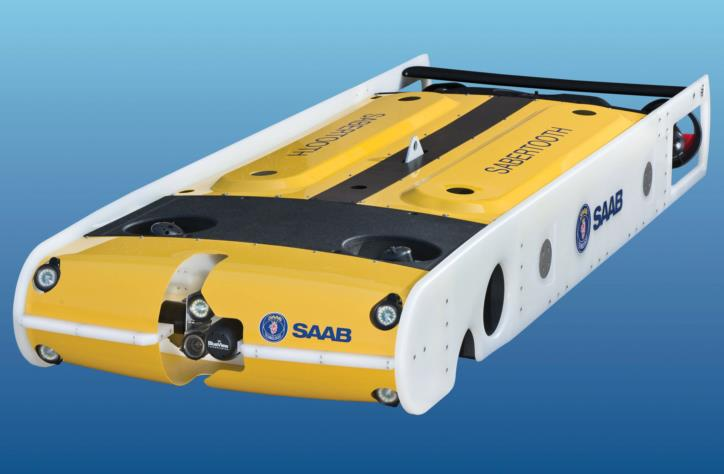
\includegraphics[scale=0.3]{Sabertooth}
  \captionsetup{justification=centering}
  \caption{SAAB Sabertooth}
\end{figure}

In our case, we wish to design a localization method for our vehicle, the Bumblebee AUV 2.5. This is then tested in multiple AUV competitions such as the Singapore AUV Challenge (SAUVC) and Robosub in San Diego, where tasks simulating industry and military use cases are required to be performed. Some of these tasks include having to localize and approach objects up to 15m away in murky water conditions, such as buoys which simulate mines and target boards which simulate items that an AUV has to get close enough to perform a task with it's end-effector.

\subsection{Motivation}

\begin{figure}[h!]
  \centering
  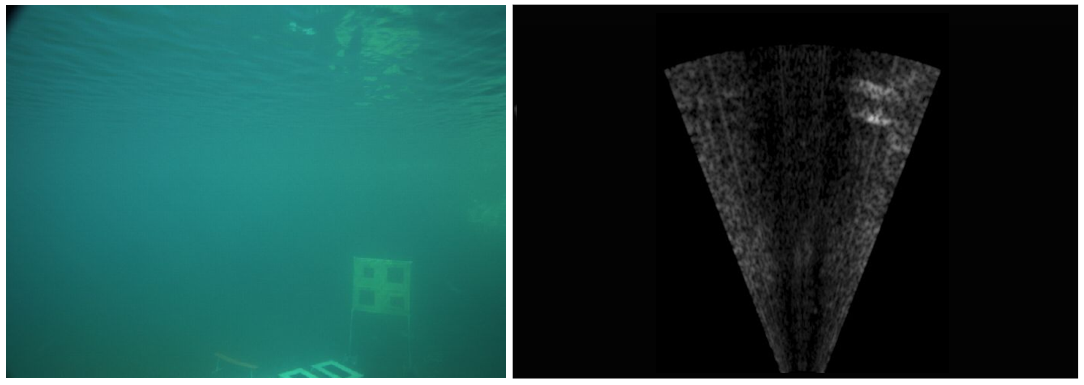
\includegraphics[scale=0.3]{pfsem1}
  \captionsetup{justification=centering}
  \caption{Objects seen in both the camera and sonar are barely visible}
\end{figure}

Optical cameras are extensively used for this purpose, where one can make use of various image processing algorithms to find a region of interest (ROI) and it's centroid (\UCamera, \VCamera) to track. However, finding this from the image alone is difficult. In shallow environments, noise can be attributed to spatio-temporal irradiance (flickering) and scattering \cite{Swirski2013}. This makes algorithms for thresholding or segmentation work ineffectively, which makes localization difficult. In deep environments, hazing due to low light conditions and suspended particles in the water make segmentation via Edge based or HSV color space based segmentation difficult. Bianco \cite{Carlevaris-Bianco2010} uses the dark channel prior estimate to dehaze the scene, and get a depth map as well, but this method cannot run in real time. Camera's are unable to perceive depth or bearing without resorting to Structure from Motion (SFM) or Stereo Camera techniques, both which require good features to track and hence are are susceptible to the issues above.

Sonars are also extensively used for this purpose. Two popular models in ROV's/AUV's are the DIDSON (Dual-Frequency Identification Sonar) and the Teledyne Blueview series, based on blazed array technology. The sonar used here is the Blueview P450-E \cite{Blueview}. It is able to provide video imagery at up to 12Hz, and has a maximum Range (\RSonar), Azimuth (\ThetaSonar), and Elevation (\PhiSonar) of 200m, 45\si{\degree} and 15\si{\degree} respectively.  Similar algorithms are used to extract Range (\RSonar) and Azimuth (\ThetaSonar) of objects from the sonar imagery.  However, the coarser sensor resolution combined with the lower signal-to-noise ratio (SNR) make data extraction challenging. Reflections from walls, or waves on the water surface produce large amount of noise. Objects out of the frustum of the sonar look noisy. Furthermore, most mid-range systems such as the one used here are unable to provide Elevation (\PhiSonar) data, making it impossible to compute 3D coordinates, and hence correct for depth.

\subsection{Objective}

The visibility limitations, intermittent loss of data due to high SNR and lack of 3D information of the object make localization difficult. In this paper, we propose a novel method for fusing information from the camera and sonar imagery, along with odometry information from the vehicle using particle filters to localize objects, assuming prior information such as the dimensions and color of said object is provided.

This paper assumes that both sensors are arranged with overlapping views, and hence it would be possible to model the transformational geometry between both spaces. It assumes that sonar is factory calibrated, and that a pre-calibration step on the camera is performed to find it's intrinsic matrix. The premise is to acquire (\RSonar, \ThetaSonar) and (\UCamera, \VCamera) from the sonar and camera data to compute the 3D coordinates (\XSonar, \YSonar, \ZSonar) in the sonar frame, which is then used for path planning purposes. Lastly, it assumes that odometry information, such as angles of rotation (\RollVehicle, \PitchVehicle, \YawVehicle), angular velocities (\RollVehicleVelocity, \PitchVehicleVelocity, \YawVehicleVelocity), translational velocities (\XVehicleVelocity, \YVehicleVelocity, \ZVehicleVelocity), and depth (\Depth) from the water surface are known, possibly through the use of a Doppler Velocity Log (DVL), Inertial Measurement Unit (IMU), and pressure sensor about the vehicle center of mass (COM). These are assumed to be calibrated as well. 

\section{Literature Review}

\subsection{Existing Approaches}
Many previous sensor fusion approaches that used range and bearing (LIDAR, RADAR, SONAR) with an optical camera have been tested and used well-defined environments with many features to track, where the sonar points towards the surface but not ahead \cite{Williams2004} \cite{Xu2012}. In the seminal paper describing 3D mapping of the great barrier reef \cite{Williams2004}, the transformations between the sensors appear to be already known/calibrated, and particle filters are used here in the SLAM process, where the motion model of the particles use vehicle odometry data. The bottom camera feed has significant features to track in order to perceive range and is at close proximity to the objects of interest. This might not be the case in the forward range where objects are much further away with poor visibility. However, many useful ideas, such as projection of the sonar features into the camera frame, and involvement of vehicular odometry in localizing stationary objects are later used in this paper.

\begin{figure}[h!]
  \centering
  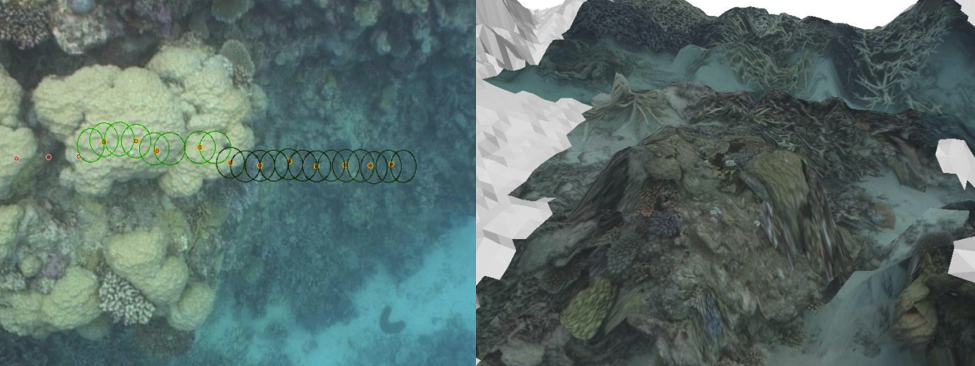
\includegraphics[scale=0.5]{reef}
  \captionsetup{justification=centering}
  \caption{Great Barrier Reef 3D mapping in William's paper}
\end{figure}

Since the FLS does not provide elevation information, methods such as projecting the sonar ambiguity space has also been explored. In Anthony Spear’s paper \cite{Spears}, where the use case was for localizing underwater ice systems in the Antarctic regions, objects detected in the sonar data are mapped directly into the camera image as an area of interest in which to search for landmarks. Although a precise calibration method is not used here, the field of view of both sensors are used to determine a bounding box where the object may exist in the camera frame. Such ideas were used in the paper as well. However, this method may not have been enough to localize precisely or acquire said objects 3D coordinates.

\begin{figure}[h!]
  \centering
  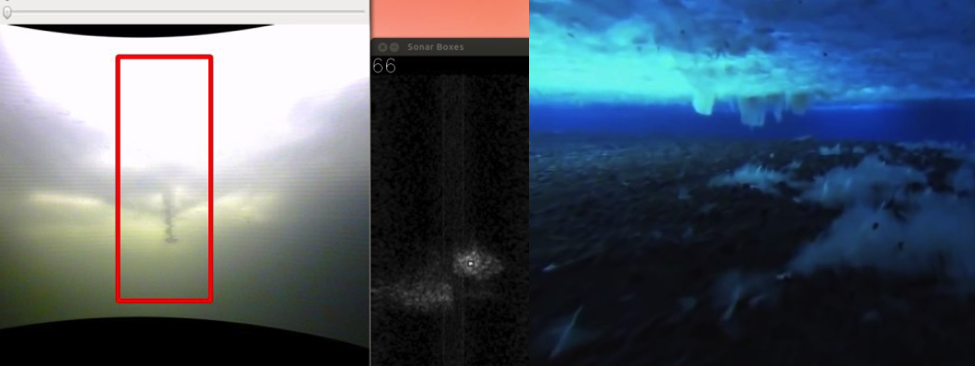
\includegraphics[scale=0.5]{ice}
  \captionsetup{justification=centering}
  \caption{Projecting sonar image into camera space on under ice topography in Spear's paper}
\end{figure}

Motion tracking approaches fusing information from sonar and camera data using a Joint Probabilistic Data Association (JDPA) fusion approach has also been studied \cite{Krout2011}. Information from the camera is used to correct the position of the floating buoy in a planar space. This method works well as the camera is on the surface, allowing better tracking on that space. However, our use case requires the system to localize objects in 3D space while fully submerged, and fusion in 2D space may only aid in visual servoing which is not the intention.

\begin{figure}[h!]
  \centering
  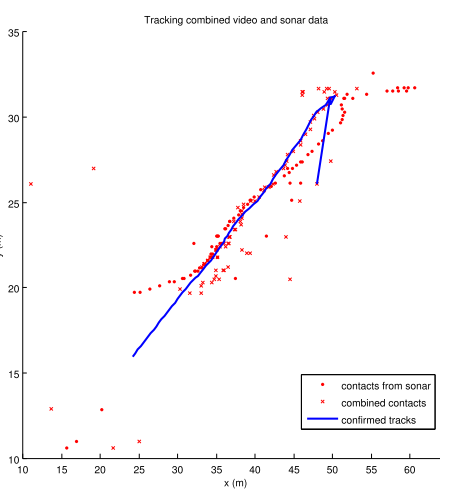
\includegraphics[scale=0.4]{jdpa}
  \captionsetup{justification=centering}
  \caption{JDPA tracking in Krout's paper}
\end{figure}

SLAM approaches using particle filters in underwater environment \cite{Clark2007}, and AUV Rigid body dynamics \cite{Miller2010} have also been studied. Clark's paper talks about the use of a PHD particle filter on FLS data, incorporating a dynamic model based on velocity and a measurement model based on intensity and centroids of thresholded objects in the sonar imagery. Miller's paper talks about the dynamic model used in a particle filter to incorporate data from the AUV's pressure sensors, DVL, IMU and an Acoustic Long Baseline (ALB). Ideas from the measurement models used in Clark's paper and vehicular dynamic models in Miller's paper are later used.

\begin{figure}[h!]
  \centering
  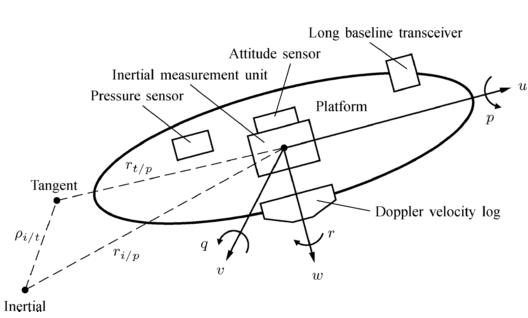
\includegraphics[scale=0.4]{vmodel}
  \captionsetup{justification=centering}
  \caption{AUV Dynamic model in Miller's paper}
\end{figure}

Lastly, state of the art calibration techniques between sonar and camera spaces by S. Negahdaripour have also been extensively studied \cite{Negahdaripour2009} \cite{Negahdaripour2010}. In these papers, opti-acoustic feature matching and the epipolar geometry between both sensors is discussed. The equations describing both sensor spaces include the polar to cartesian conversions of the sonar space, transformation matrix between both sensors, perspective projection of 3D points into the camera space as pixels and a closed formed solution solving for \PhiSonar. The paper describes the use of the Levenberg Marquardt algorithm \cite{marquardt:1963} for non-linear optimization in order to solve for the unknown transformation parameters, and also shows the use of a special calibration grid. Although a much simplified model is used later on for our use case, many ideas are taken from these two papers.

\begin{figure}[h!]
  \centering
  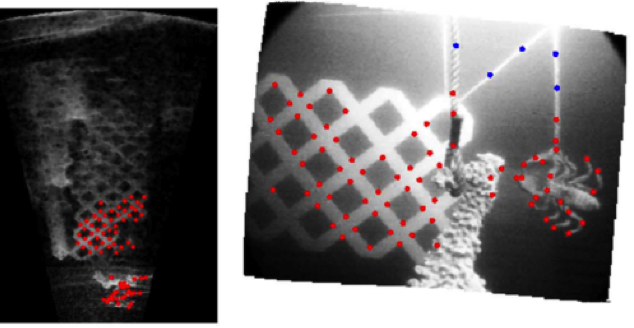
\includegraphics[scale=0.3]{sonarcam}
  \captionsetup{justification=centering}
  \caption{Corresponding points between sonar and camera images in Negahdaripour's paper}
\end{figure}

In the above approaches, methods that involved fusion of both sensors had the availability of a rich set of features to track, due to certain sensors being out of the water, or being in close proximity with the floor. In our scenario however, we are required to localize objects in front of the AUV at ranges of up to 15m, and we may not have this luxury. Furthermore, at those ranges, the minimal features that we do track in both sensors may have large errors without proper calibration. In all of the above approaches, we are yet to find a method that achieves centimetre level accuracy at those ranges, where camera, sonar and vehicular dynamics are all used to localize objects in front of the AUV, through the use of statistical filters. In order to achieve our objectives, we aim to fill this gap.

\subsection{Vehicle Used}

\begin{figure}[h!]
  \centering
  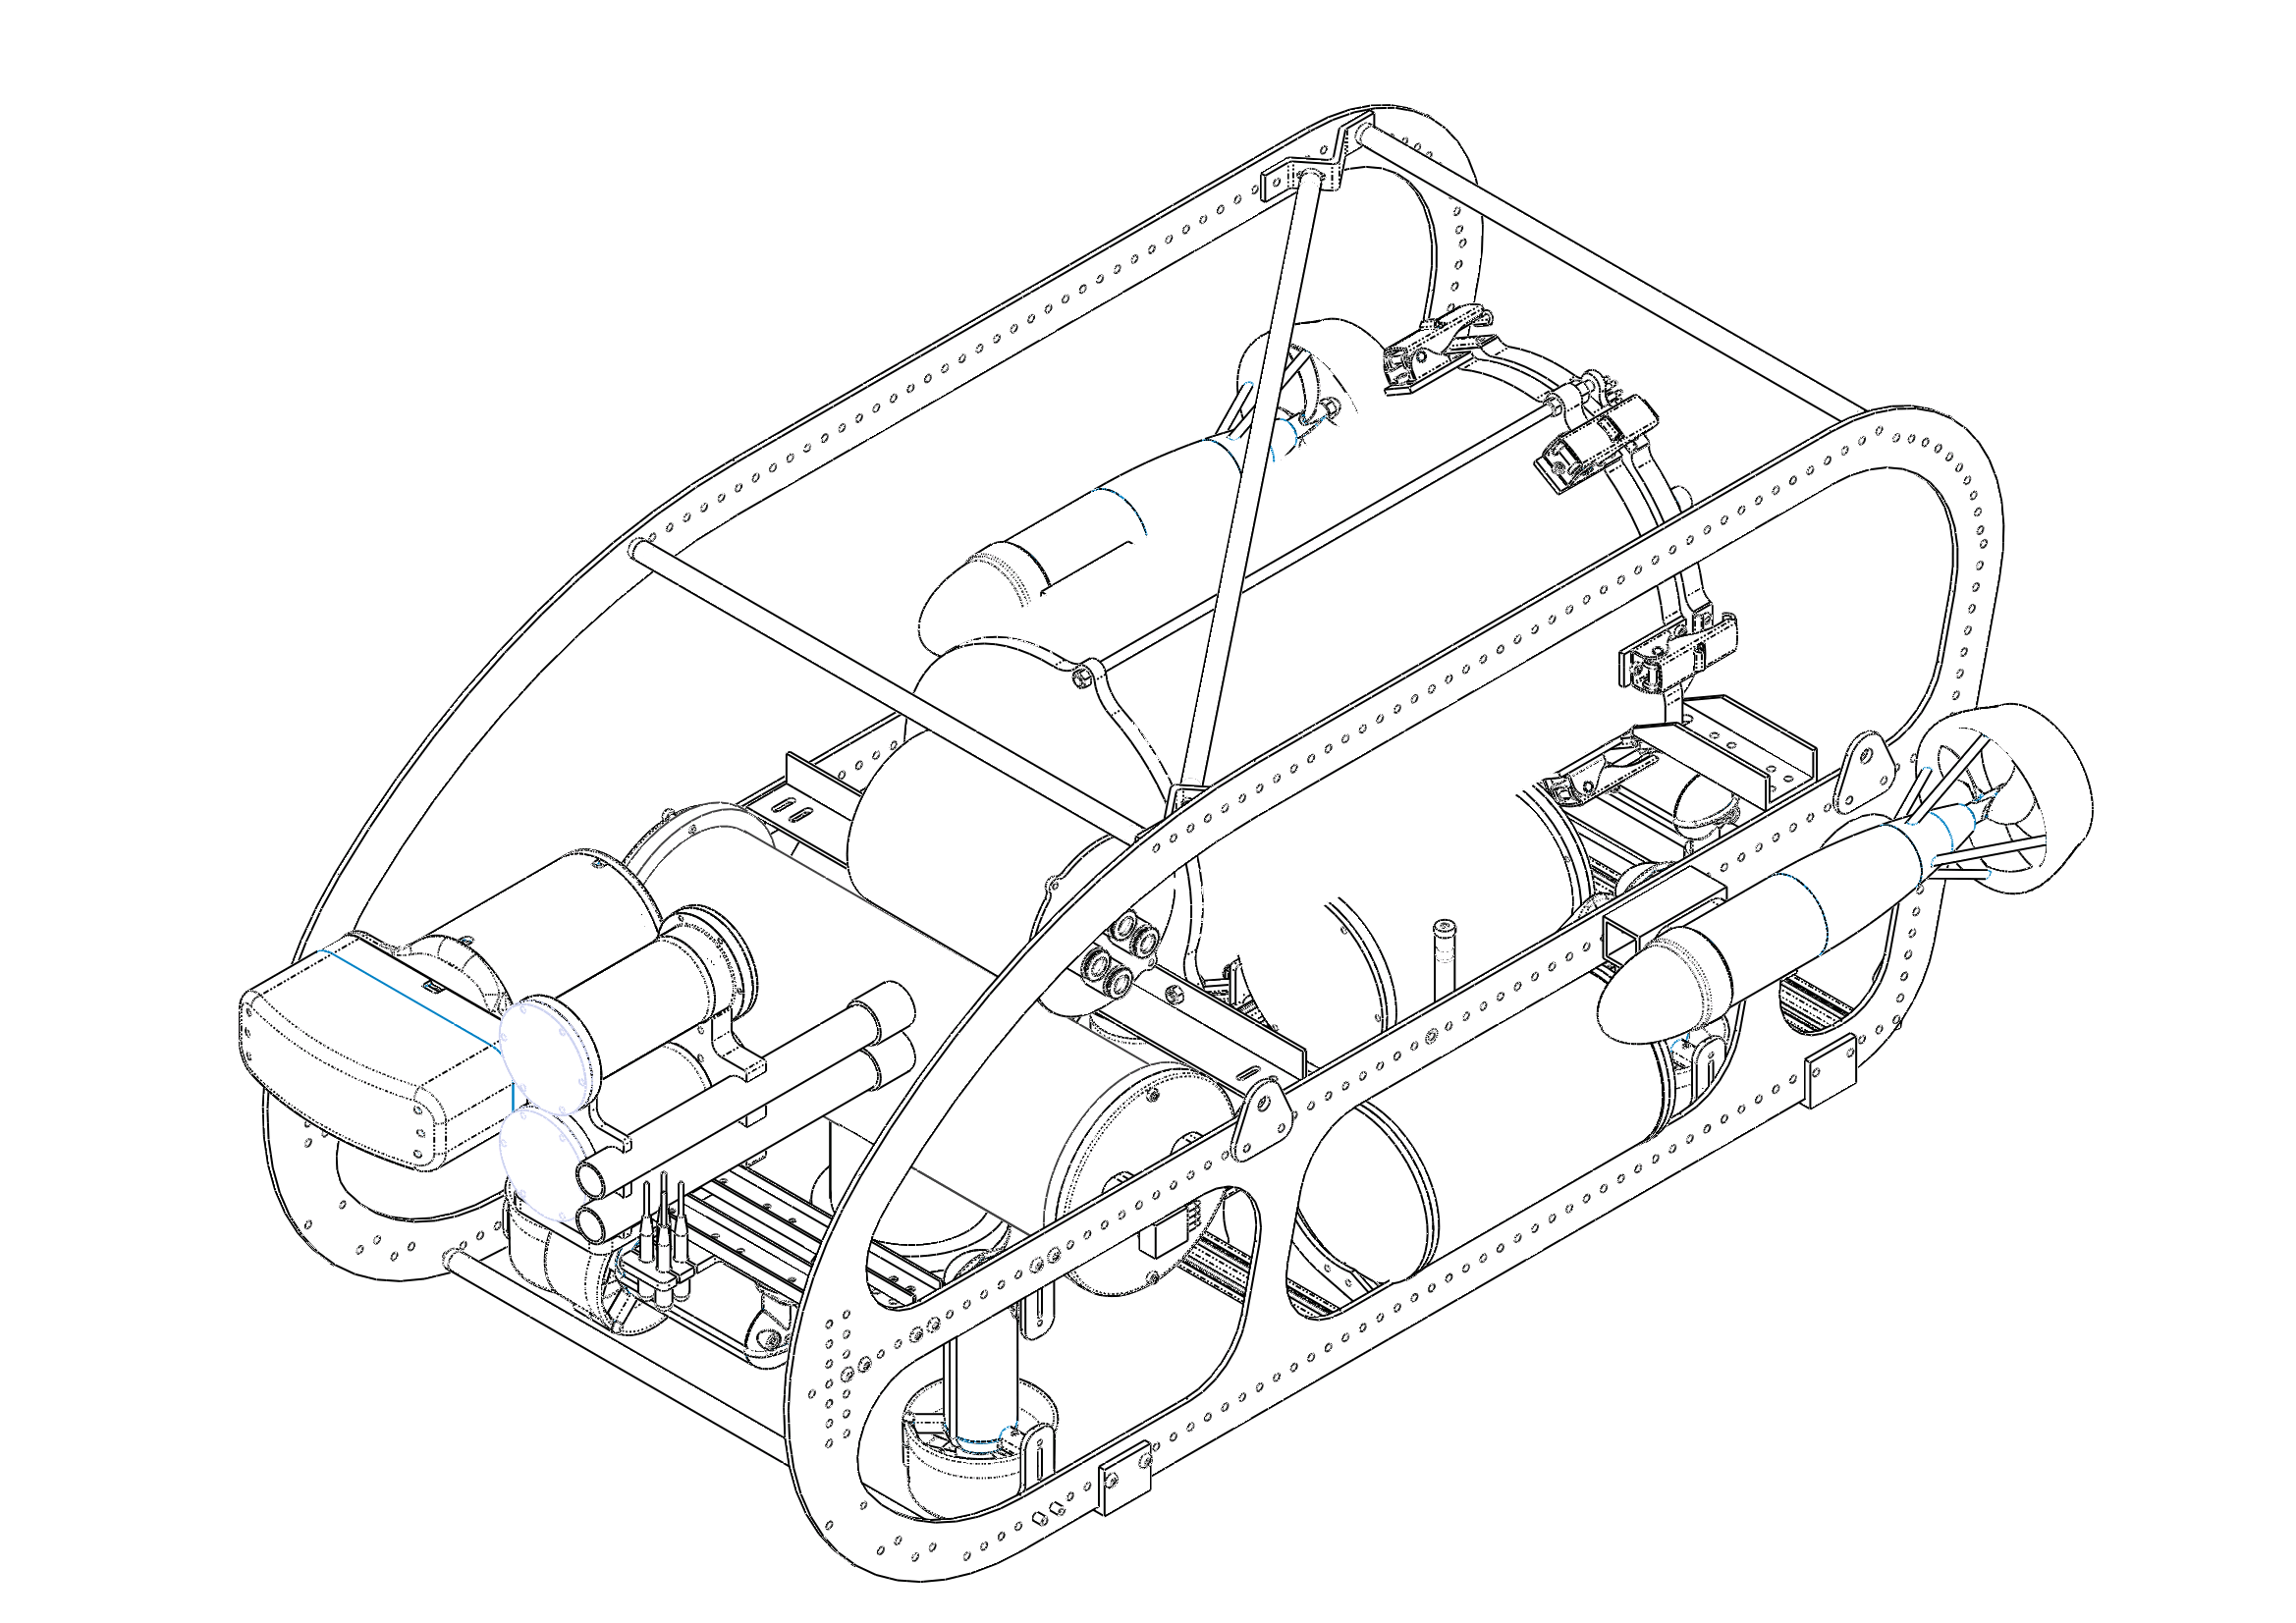
\includegraphics[scale=0.2]{bbauv25}
  \captionsetup{justification=centering}
  \caption{BumbleBee AUV 2.5}
\end{figure}

\begin{table}[h]
\centering
\begin{tabular}{|l|l|}
\hline
{\bf Weight}                & 50 kg                                                                                                                \\ \hline
{\bf Dimensions}            & 0.7m X 1.1m X 0.5m                                                                                                   \\ \hline
{\bf Single Board Computer} & \begin{tabular}[c]{@{}l@{}}Core i7 - 3610QE\\ Aaeon EMB-QM77\\ 8GB DDR3 RAM\\ 512GB SATA3 SSD\end{tabular}           \\ \hline
{\bf Embedded System}       & \begin{tabular}[c]{@{}l@{}}Arduino Mega 2560\\ Xilinx Spartan-3 on NI sbRIO 9602\end{tabular}                        \\ \hline
{\bf Propulsion}            & \begin{tabular}[c]{@{}l@{}}6 SeaBotix BTD150\\ 2 VideoRay Surge Thrusters\end{tabular}                               \\ \hline
{\bf Navigation}            & \begin{tabular}[c]{@{}l@{}}Teledyne RDI Explorer DVL\\ Sparton GEDC-6 IMU\\ US300 Pressure/Depth Sensor\end{tabular} \\ \hline
{\bf Vision Sensors}        & \begin{tabular}[c]{@{}l@{}}AVT Guppy Pro\\ AVT Guppy\end{tabular}                                                    \\ \hline
{\bf Sonar}                 & \begin{tabular}[c]{@{}l@{}}BlueView P450 Imaging Sonar\\ 4 Teledyne Reson TC4013 Hydrophones\end{tabular}            \\ \hline
{\bf Manipulators}          & Festo Pneumatics Systems                                                                                             \\ \hline
{\bf Power Supply}          & 22.2V 10000mAh LiPo Battery (x2)                                                                                      \\ \hline
{\bf Underwater Connectors} & SubConn Micro and Low Profile Series                                                                                 \\ \hline
{\bf Software Architecture} & \begin{tabular}[c]{@{}l@{}}Robot Operating System (ROS)\\ Debian GNU/Linux x64\end{tabular}                          \\ \hline
\end{tabular}
\caption{BumbleBee AUV 2.5 Specifications}
\end{table}

The vehicle used for testing is the Bumblebee Autonomous Underwater Vehicle (BBAUV) \cite{BBAUV}. BBAUV is equipped with a Guppy Pro F-503 5 Megapixel Color CMOS Camera, Blueview P450-E Imaging Sonar for vision, Teledyne TDI Explorer DVL (Doppler Velocity Log), Sparton AHRS-8 IMU, Reson TC4013 hydrophones and a depth sensor for navigation and acoustics, and 2 VideoRay and 6 SeaBotix Thrusters for up to 6DOF. Fusion of the DVL and IMU via an Extended Kalman Filter provides odometry information and allows the vehicle to move to any 3D Coordinate. The US300 pressure depth sensor provides depth with an accuracy of +-1cm. The sonar, camera and odometry sensors lie in the same rigid body frame where the transformations between them is known through the mechanical model. This information will be later used as initial values for the calibration process.

\subsection{Sonar Model}

\begin{figure}[h!]
  \centering
  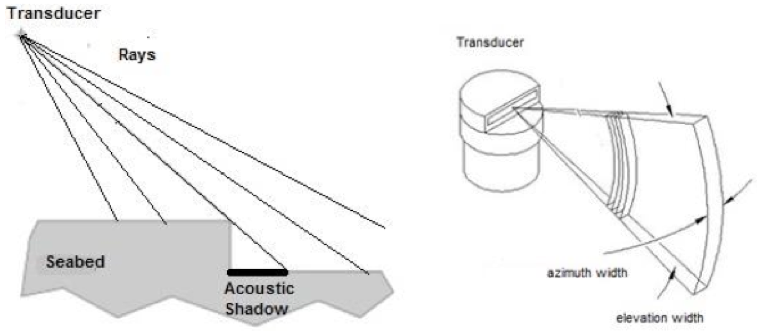
\includegraphics[scale=0.3]{sonar3}
  \captionsetup{justification=centering}
  \caption{FLS Image Formation 1}
\end{figure}

Concepts and equations behind the FLS are based off the “Springer handbook of robotics” \cite{handbook-of-robotics} while understanding of formation of FLS imagery is based off \cite{Coiras2009}. An FLS is made of an array of vertical and horizontal transducers, which generate pulses of high frequency noise (450 Khz for the P450-E). The FLS Model is usually represented in spherical coordinates of azimuth, elevation angles, and range. They are also equipped with multiple transducers (The P450-E has 256 transducers). Each individual transducer can be represented as an optical ray, where the azimuth and elevation are 1\si{\degree} and 15\si{\degree} respectively as seen from Fig. 9. Hence, the horizontal beam spacing is about 256/45=0.18\si{\degree}. 

Sonar’s form images using time of flight of pulses. Each transducer output/ray can be plotted as a function of time which consists of both Intensity and Range as seen from Fig. 10. Objects that are further away have a lower intensity due to signal attenuation in the medium. Also, there is a possibility that two objects at different \PhiSonar but same \RSonar may overlap in the image causing it to be impossible to perceive both objects separately. Furthermore, reflections from walls may result in objects appearing further than they actually are.

\begin{figure}[h!]
  \centering
  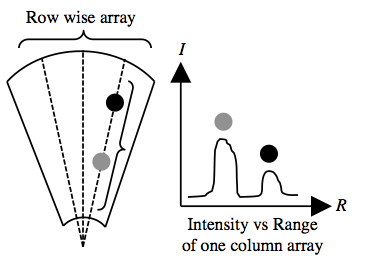
\includegraphics[scale=0.5]{transducers}
  \captionsetup{justification=centering}
  \caption{FLS Image Formation 2}
\end{figure}

Intensity of the object is also dependant on the angular deviation from the line-of-sight of the transducer \cite{Creuze2005}.  $\lambda$ is the sound wavelength, a and b are the length and the width of the aperture of the transducer respectively, $\alpha$ and $\beta$ are the coordinates of the vector of angular deviation and Io(R) is the sound intensity at range R on the beam axis as seen from Eq. 1. Assuming the vehicle has an operating depth of less than 100m, based on the depth profile, it would have a $\lambda$ of 450khz/1500 = 0.003m.
\begin{gather}
I\left( R,\theta  \right)\; =\; I_{0}\left( R \right)\left( \frac{\sin \; p}{p} \right)^{2}\left( \frac{\sin \; q}{q} \right)^{2} \\
p\; =\; \frac{\pi a\alpha }{\lambda }\; q\; =\; \frac{\pi b\beta }{\lambda }\; 
\end{gather}
 
Lastly, the geometry of the object can be represented by Fig. 11 and Eq. 3. Here, we represent the sonar frame and the object coordinates in that frame in both cartesian and polar form. An alternative form is also used in this case, as the sensor inputs to form the 3D position of the object happen to be \RSonar, \ThetaSonar and \YSonar. \PhiSonar is not a sensor output provided by the sonar and is actually a value we wish to solve for later in the paper.
\begin{gather}
\left[ \begin{array}{c} X_{s} \\ Y_{s} \\ Z_{s} \end{array} \right]\; =\; \left[ \begin{array}{c} R_{s}\cdot \cos \left( \phi _{s} \right)\cdot \sin \left( \theta _{s\; } \right) \\ R_{s}\cdot \sin \left( \phi _{s} \right) \\ R_{s}\cdot \cos \left( \phi _{s} \right)\cdot \cos \left( \theta _{s\; } \right) \end{array} \right]\; =\; \left[ \begin{array}{c} \sqrt{R_{s}^{2}\; -\; Y_{s}^{2}}\cdot \sin \left( \theta _{s\; } \right) \\ Y_{s} \\ \sqrt{R_{s}^{2}\; -\; Y_{s}^{2}}\cdot \cos \left( \theta _{s\; } \right) \end{array} \right]\; 
\end{gather}

\begin{figure}[h!]
  \centering
  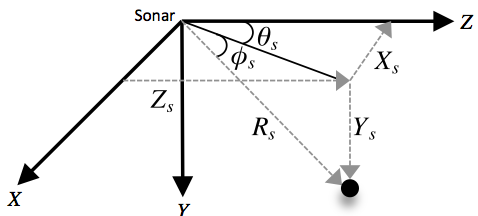
\includegraphics[scale=0.4]{sonarframe}
  \captionsetup{justification=centering}
  \caption{Sonar Frame}
\end{figure}

\subsection{Camera Model}

\begin{figure}[h!]
  \centering
  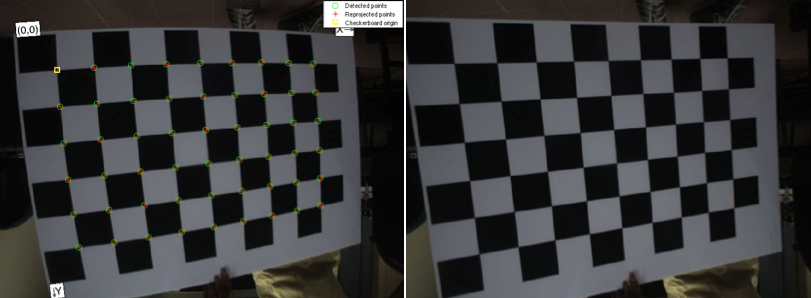
\includegraphics[scale=0.3]{camera}
  \captionsetup{justification=centering}
  \caption{Camera Calibration}
\end{figure}

The camera is geometrically calibrated via Zhang’s method \cite{Sturm1999} using a checkerboard pattern. Multiple checkboards images are used, and are used to estimate the camera’s distortion parameters and instrinsic matrix. This allows us to map real world coordinates onto the camera plane by finding the focal lengths and principal points as seen in Eq. 4. To account for camera distortion, the radial coefficients (K Values) are also estimated using Brown-Conrady model as seen in Eq. 6. The results and the equations used are are shown below:
\begin{gather}
\left[\begin{array}{c}
U_{c}\\
V_{c}
\end{array}\right]=\left[\begin{array}{cccc}
f_{x} & 0 & c_{x} & 0\\
0 & f_{y} & c_{y} & 0\\
0 & 0 & 1 & 0
\end{array}\right]*\left[\begin{array}{c}
X_{c}\\
Y_{c}\\
Z_{c}\\
1
\end{array}\right]=>\left[\begin{array}{c}
\frac{(f_{x}*X_{c})+(c_{x}*Z_{c})}{Z_{c}}\\
\frac{(f_{y}*Y_{c})+(c_{y}*Z_{c})}{Z_{c}}
\end{array}\right] \\
r=\sqrt{((U_{D}-c_{x})/f_{x})^{2}+((V_{D}-c_{y})/f_{y})^{2}} \\
\left[\begin{array}{c}
U_{U}\\
V_{U}
\end{array}\right]=\left[\begin{array}{c}
f_{x}*(((U_{D}-c_{x})/f_{x})*(1+K_{1}*r^{2}+K_{2}*r^{4}))+c_{x}\\
f_{y}*(((V_{D}-c_{y})/f_{y})*(1+K_{1}*r^{2}+K_{2}*r^{4}))+c_{y}
\end{array}\right]
\end{gather}

\subsection{Estimation Theory}

Estimation theory is widely used in many robotics applications. The problem is to sequentially estimate the state of a dynamic system (in this case our object to be localized) using noisy measurements from our various sensors. We have a state vector that contains all information required to describe the system (Eg. position and velocity of the object w.r.t the vehicle in 3D space), and we have a measurement vector that contain observations that a related to the state vector through some model (Eg. range and azimuth from the sonar image). A dynamic model is used to describe the system dynamics, such as predicting the next position of an object, and a measurement model is used to relate the measurement and state vectors. Much of the theory and equations used is extracted from Trieb's paper \cite{Trieb2005}.

One way to describe these models is through a Recursive Bayesian Filter, which consists of a prediction and an update stage and assumes the state's uncertainty is distributed through a Gaussian distribution. The prediction step predicts the next pdf using the dynamic model, but uncertainty is added due to system noise (Eg. using odometry data to predict the object's next position has noise), hence stretches the distribution. The update stage then squeezes the distribution using Bayes' theorem. These steps can be described in Eq. 7/8 where $s_{k}$ is the state of the system at time $k$, $f$ is the dynamic model with process noise $w_{k}$ that is used to predict the next state $s_{k+1}$. $h$ is the measurement model with measurement noise $v_{k}$ that is used to correct $s_{k}$.
\begin{gather}
s_{k+1}=f(s_{k},w_{k})\quad k\epsilon\mathbb{N} \\
z_{k}=h(s_{k},v_{k})\quad k\epsilon\mathbb{N}
\end{gather}

Given a set of prior observations up to a time $k$, we wish to find the optimal estimate for $s_{k}$. If $p(s_{k}|Z_{k-1})$ is known, the correction step of the pdf can be derived as seen in Eq. 10. If $p(s_{k}|Z_{k})$ is known, the prediction step of the pdf can be derived as seen in Eq. 11. 
\begin{gather}
Z_{k}=\{z_{0},...,z_{k}\}=\{Z_{k-1},z_{k}\} \\
p(s_{k}|Z_{k})=\frac{p(Z_{k}|s_{k})p(s_{k})}{p(Z_{k})}=\frac{p(z_{k},Z_{k-1}|s_{k})p(s_{k})}{p(z_{k},Z_{k-1})} \nonumber\\
=\frac{p(z_{k}|s_{k},Z_{k-1})p(Z_{k-1}|s_{k})p(s_{k})}{p(z_{k}|Z_{k-1})p(Z_{k-1})}=\frac{p(z_{k}|s_{k})p(Z_{k-1}|s_{k})p(s_{k})}{p(z_{k}|Z_{k-1})p(Z_{k-1})} \nonumber\\
=\frac{p(z_{k}|s_{k})p(s_{k}|Z_{k-1})}{p(z_{k}|Z_{k-1})} \\
p(s_{k+1},s_{k}|Z_{k})=p(s_{k+1}|s_{k},Z_{k})p(s_{k}|Z_{k})=p(s_{k+1}|s_{k})p(s_{k}|Z_{k}) \nonumber\\
p(s_{k+1}|Z_{k})=\int_{\mathbb{R^{\mathit{n}}}}p(s_{k+1}|s_{k})p(s_{k}|Z_{k})ds_{k}
\end{gather}

The recursive propagation of the pdf can only be done if the system is linear and gaussian, which might not be the case for us. To account for this, one way would be to linearise the system then applying a Kalman Filter (Extended Kalman Filter EKF).

The Kalman Filter assumes that the pdf at every time step is Gaussian, and can be described by a mean and covariance. If we assume the dynamic and measurement models are linear with some gaussian noise added, the filter can be described based on these Eq. 12/13 where $F_{k}$ and $H_{k}$ describe the dynamic and measurement models as linear functions, $w_{k}$, $v_{k}$ and $s_{0}$ are normally distributed based on Eq. 14. 
\begin{gather}
s_{k+1}=F_{k}s_{k}+G_{k}w_{k}\quad k\epsilon\mathbb{N} \\
z_{k}=H_{k}s_{k}+v_{k}\quad k\epsilon\mathbb{N} \\
w_{k}\sim N(0,Q_{k}),\quad v_{k}\sim N(0,R_{k}),\quad s_{0}\sim N(\hat{x}_{0},P_{0})
\end{gather}

The Kalman Filter proves that when $Z_{k}$ is given, $s_{k}$ and $s_{k+1}$ are distributed according to Eq. 15/16, and the filter steps is given by Eq. 17. This allows one to recursively compute the mean and covariance of the next state given that the system is linear and gaussian to begin with.
\begin{gather}
p(s_{k}|Z_{k})\sim N(\hat{s}_{k|k},P_{k|k}) \\
p(s_{k+1}|Z_{k})\sim N(\hat{s}_{k+1|k},P_{k+1|k}) \\
\hat{s}_{k|k}=\hat{s}_{k|k-1}+P_{k|k-1}H_{k}^{T}S_{k}^{-1}(z_{k}-H_{k}\hat{s}_{k|k-1}) \nonumber\\
P_{k|k}=P_{k|k-1}-P_{k|k-1}H_{k}^{T}S_{k}^{-1}H_{k}P_{k|k-1} \nonumber\\
S_{k}=R_{k}+H_{k}P_{k|k-1}H_{k}^{T} \nonumber\\
\hat{s}_{k+1|k}=F_{k}\hat{s}_{k|k} \nonumber\\
P_{k+1|k}=F_{k}P_{k|k}F_{k}^{T}+W_{k}Q_{k}W_{k}^{T}
\end{gather}

In a nonlinear non-gaussian model, one approach would be to use a particle filter. Here, the pdf is represented as a set of samples with weights. Similar to the first two methods, a dynamic model and a measurement model is used, along with the process and measurement noise. Here however, Monte Carlo (MC) methods are used where the objective is to approximate integrals of the form based on Eq. 18 where $p(s)$ represents a probability function that sums to 1. If we can draw N samples according to $p(s)$, then the integral can be approximated by the sum based on Eq. 19. As $N$ approaches infinity, we can describe the pdf more precisely and we approach an optimal Bayesian estimate. As seen in Fig. 13, particles are able to model multivariate distributions through uneven partitioning, and regions of high/low density.
\begin{gather}
I=\int g(s)p(s)ds \\
\hat{I}=\frac{1}{N}\sum_{i=1}^{N}g(s^{i})
\end{gather}

\begin{figure}[h!]
  \centering
  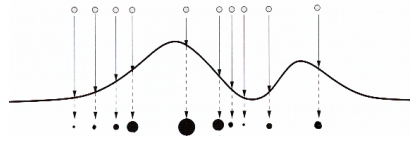
\includegraphics[scale=0.3]{particles}
  \captionsetup{justification=centering}
  \caption{Particle filter estimating pdf}
\end{figure}

\subsection{Particle Filter Algorithm}
\begin{algorithmic}[1]
\STATE \textit{Initialisation} : \\
Generate $N$ particles according to an initial distribution $p_{0}(s_{0})$ set by the user. If not set, assume a uniform distribution over a bounded space.
\STATE \textit{Dynamic Model update} : \\
Time evolution of particles occurs through the dynamic model, with process noise added in.\\
$X_{n|n-1}^{(k)}=f(X_{n-1|n-1}^{(k)},w_{n-1})\quad k\epsilon\mathbb{N}$\\
\STATE \textit{Redistribution} : \\
A certain percentage of particles are randomly selected and then uniformly distributed over the workspace to solve the captured robot problem as suggested by Sebastian Thrun's paper \cite{Fox1999}.
\STATE \textit{Measurement Model update} : \\
Compute weights for each particle given a measurement $Y_{n}$ and normalize \\
$q_{n}=\frac{P(Y_{n}|X_{n|n-1}^{(k)})}{\sum_{k}P(Y_{n}|X_{n|n-1}^{(k)})}\quad k\epsilon\mathbb{N}$
\STATE \textit{Resample} : \\
Generate $N$ new particles by resampling with replacement given a weight $q_{n}$ \\
$X_{n+1|n}^{(k)}=h(X_{n|n}^{(k)}|q_{n})\quad k\epsilon\mathbb{N}$ \\
\STATE Go to step 2 and repeat with new inputs
\end{algorithmic} 

The above steps can be described in Fig. 14 \cite{PFDemo}, where prediction is done through the dynamic model update in Step. 2/3, calculation and normalization of weights based on the measurement model in Step 4, and resampling in Step 5, in this case done using the computed likelihood histogram based on the normalized weights.

\begin{figure}[h!]
  \centering
  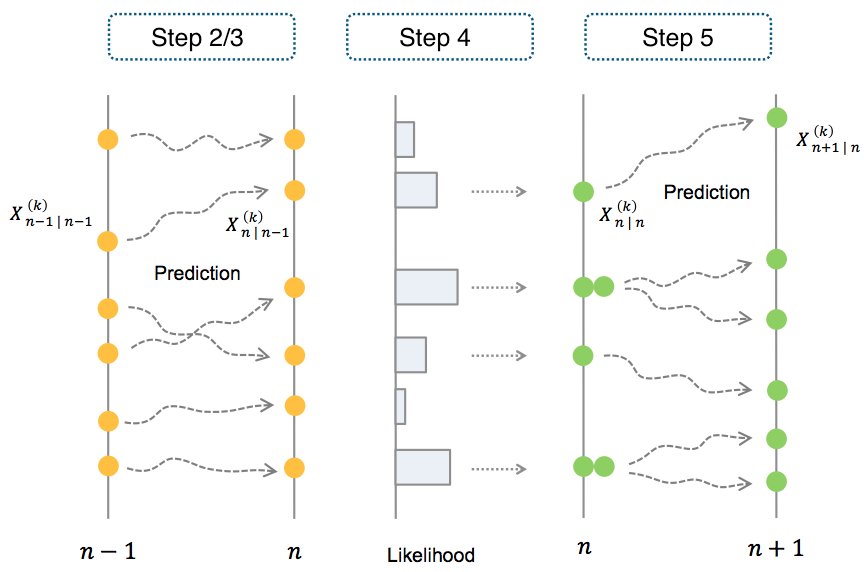
\includegraphics[scale=0.3]{resample}
  \captionsetup{justification=centering}
  \caption{Particle Filter Stages}
\end{figure}

\section{Calibration}

\subsection{Calibration Model}

\begin{figure}[h!]
  \centering
  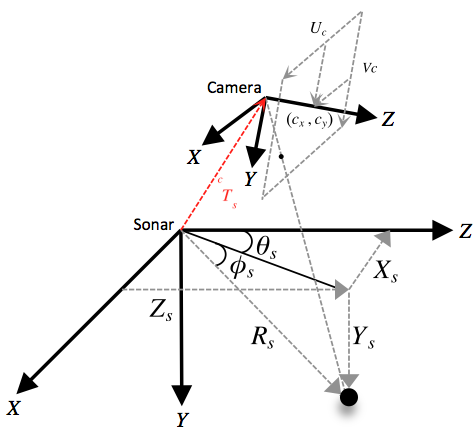
\includegraphics[scale=0.4]{sonarcamframe}
  \captionsetup{justification=centering}
  \caption{Sonar Camera Model}
\end{figure}

Now that we have an equation that can map 3D coordinates in the camera frame to camera pixels, we are able to combine both spaces as seen in Fig. 15 and Eq. 20. This assumes that we know $^{c}T_{s}$ which may be roughly estimated from physical measurements. 
\begin{gather}
\left[\begin{array}{c}
U_{c}\\
V_{c}
\end{array}\right]<=\left[\begin{array}{cccc}
f_{x} & 0 & c_{x} & 0\\
0 & f_{y} & c_{y} & 0\\
0 & 0 & 1 & 0
\end{array}\right]*
\left[\begin{array}{cccc}
^{c}T_{s11} & ^{c}T_{s12} & ^{c}T_{s13} & ^{c}T_{s14}\\
^{c}T_{s21} & ^{c}T_{s22} & ^{c}T_{s23} & ^{c}T_{s24}\\
^{c}T_{s31} & ^{c}T_{s32} & ^{c}T_{s33} & ^{c}T_{s34}\\
0 & 0 & 0 & 1
\end{array}\right]
*\left[\begin{array}{c}
\sqrt{R_{s}^{2}-Y_{s}^{2}}\cdot\sin\left(\theta_{s}\right)\\
Y_{s}\\
\sqrt{R_{s}^{2}-Y_{s}^{2}}\cdot\cos\left(\theta_{s}\right)\\
1
\end{array}\right]
\end{gather}

\begin{figure}[h!]
  \centering
  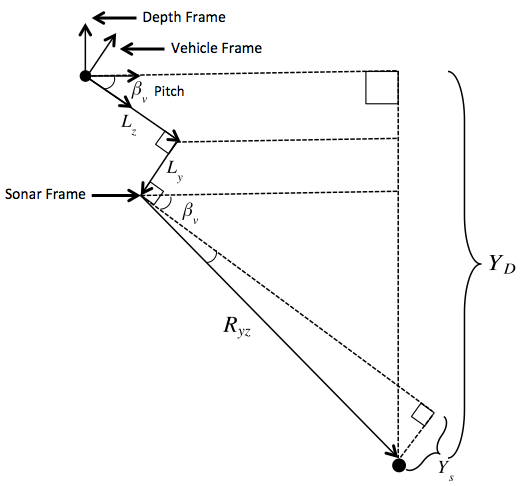
\includegraphics[scale=0.4]{sonarvehframe}
  \captionsetup{justification=centering}
  \caption{Sonar Vehicle Model}
\end{figure}

The depth sensor is located about the vehicle center of mass (COM). Assuming the depth of the object of interest is measured, and the depth of the vehicle (\Depth) is known, we can easily derive the depth of the object relative to the vehicle COM aligned to the water surface (\YDepth). The depth sensor's output is assumed to be impervious to vehicular dynamics as it is placed at the vehicle COM, and it's frame is assumed to be aligned to the water surface. Using geometrical methods, we derived an equation that approximately maps \YDepth to \YSonar and vice-versa based on Fig. 16 and Eq. 22/23 using \RSonar and \PitchVehicle. $L_{z}$ and $L_{y}$ can also be estimated from physical measurements. ($R_{yz}$) is the flattened range of the $Y_{s}$ and $Z_{s}$ axis on the sonar frame and is approximately equal to $(R_{s}*\Theta_{s})$. Based on a workspace of a max $R$ of 15m and the sonar parameters listed in Eq. 21, this approximation yields a maximum error of 1.35cm and is deemed acceptable. Also, this model assumes that the roll effect is minimal which was the case in our vehicle. The downside of this model is that we cannot estimate $L_{x}$, but we do not need it for our calibration step.
\begin{gather}
\left[\begin{array}{c}
\max\left(R_{s}\right)=15\\
\max\left(\theta_{s}\right)=45/2\\
\max\left(\phi_{s}\right)=15/2
\end{array}\right]\quad R_{yz}=R_{s}*cos(\Theta_{s})\\
Y_{D}=L_{y}*\cos\left(\beta_{v}\right)+L_{z}*\sin\left(\beta_{v}\right)+R_{yz}*\sin\left(\beta_{v}+\mbox{asin}\left(\frac{Y_{s}}{R_{yz}}\right)\right) \\
Y_{s}=-R_{yz}*\sin\left(\beta_{v}+\mbox{asin}\left(\frac{\left(L_{y}*\cos\left(\beta_{v}\right)-Y_{D}+L_{z}*\sin\left(\beta_{v}\right)\right)}{R_{yz}}\right)\right)
\end{gather}

From these models, we are able to derive a closed form solution that allows one to compute \YSonar and hence calculate \PhiSonar from (\PitchVehicle, \RSonar, \ThetaSonar, \UCamera and \VCamera).  It also allows us to compute \UCamera and \VCamera from \YDepth, \PitchVehicle, \RSonar and \ThetaSonar if the depth of the object is known. Lastly, if the depth of the object is unknown, it allows us to compute a possible solution space since \YSonar has a min/max elevation of 15\si{\degree}.

However, this assumes that $L_{z}$, $L_{y}$ and $^{c}T_{s}$ are precise. This might not be the case from physical measurements alone. This is why calibration techniques are later used to estimate these parameters more precisely.

\subsection{Data Collection}

In order to collect data to fit into our model, we wish to extract (\RSonar, \ThetaSonar, \UCamera, \VCamera, \PitchVehicle, \YDepth) over a large range. Hence, we have to come up with an algorithm to automatically detect and collect data. This means extracting data from both the camera and the sonar imagery without human intervention using computer vision techniques. This speeds up the data collection process, and results in more accurate data. The test object used here is a solid fluid-filled yellow sphere/buoy with a radius of 0.2m. Solid sphere's are normally used in sonar calibration due to their high levels of insonification and the fact that we can take it's centroid as a single point \cite{4804062}. Also, the yellow sphere can be easily segmented in the camera image as it's hue is significantly different from the surrounding pool. The buoy's precise depth is measured by placing the depth sensor on it, allowing us to calculate \YDepth. \PitchVehicle is available from the vehicle's on-board IMU. The other information can be extracted from the images. Software used in this entire system consists of Numpy/Scipy for matrix computations \cite{dubois-1999-cse}, ROS (Robot Operating System) for communication \cite{Quigley2009}, OpenCV for image processing functions \cite{opencv_library} and MATLAB for algorithm development.

\begin{figure}[h!]
  \centering
  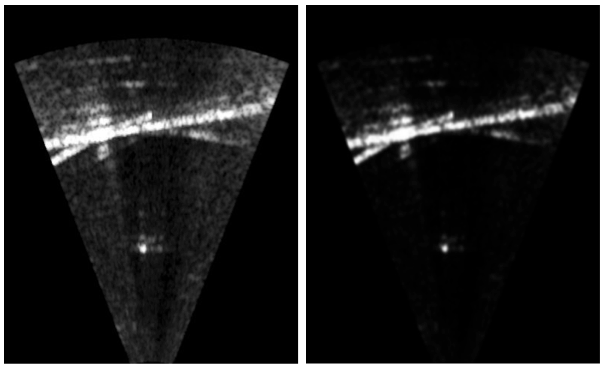
\includegraphics[scale=0.4]{sonarprocessed}
  \captionsetup{justification=centering}
  \caption{Before and after applying image processing techniques on sonar image}
\end{figure}

Figure 17 shows the image direct from the sensor and after various filters are applied. Several methods used here are referenced from Kim's paper on radar processing techniques \cite{Kim2001}. The first stage was to convolve the image with a 2-D isotropic Gaussian low pass kernel with a $\sigma $ of 5 pixels based on Eq. 24. N and M represent the width and height of the sonar image respectively. This helps remove some of the sparse electrical or acoustic noise in the image. Power law is then applied to the normalized image to enhance brighter regions based on Eq. 25. Finally, image averaging based on Eq. 26 is applied, and helps lower the intensity of sporadic noise that appears in and out of subsequent frames. 
\begin{gather}
g\left( x,y \right)\; =\; e^{\frac{-\left( \left( x-c_{x} \right)^{2}+\left( y-c_{y} \right)^{2} \right)}{\left( 2\sigma  \right)^{2}}} \\
c_{x}\; =\; 0.5\cdot N\; c_{y}\; =\; 0.5\cdot M\; \sigma =5\; \nonumber\\
I\left( x,y \right)\; =\; I\left( x,y \right)\otimes g\left( x,y \right) \nonumber\\
I\left( x,y \right)\; =\; \left( \frac{I\left( x,y \right)}{255} \right)^{2}\cdot 255 \\
I\left( x,y \right)\; =\; \frac{\sum_{i}^{2}{I\left( x,y \right)}}{2}
\end{gather}

After these image processing methods, a combination of thresholding, morphology and contour detection is used to extract objects from the image. We can easily extract and track the calibration buoy using these methods as they are distinct from other objects in the image. These  pre-processing techniques will also be later applied before more complex filters such as particle filters are applied. Once the coordinates in the sonar image are extracted, they are passed to the Blueview API to extract \RSonar and \ThetaSonar.

\begin{figure}[h!]
  \centering
  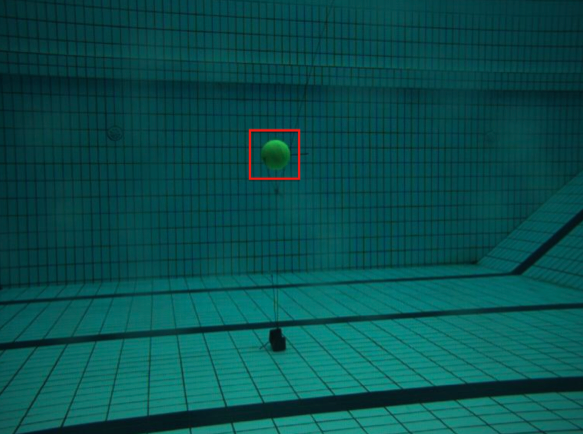
\includegraphics[scale=0.3]{buoycamera}
  \captionsetup{justification=centering}
  \caption{Calibration buoy seen in the camera frame}
\end{figure}

Camera points are extracted using contrast enhancement, HSV Thresholding to pick out yellow and morphology. This way, we can precisely extract \UCamera and \VCamera automatically. A data collection UI has also been written to extract all this information into a MATLAB friendly format.

\subsection{Calibration process}

A set of data points with (\RSonar, \ThetaSonar, \UCamera, \VCamera), (\RollVehicle, \PitchVehicle, \YawVehicle), (\RollVehicleVelocity, \PitchVehicleVelocity, \YawVehicleVelocity), (\XVehicleVelocity, \YVehicleVelocity, \ZVehicleVelocity) and \YDepth is collected over a space of 10x2.5x12 metres. A total of 10,000 points was collected over this space and split into 5 datasets consisting of 1 training set and 4 test sets. Camera calibration is conducted to solve for ($f_{x}$, $f_{y}$, $c_{x}, c_{y}$, $K_{1}$,$K_{2}$) on both land and water, and tested to see the that ($f_{x}$, $f_{y}$) differ by 1.33. $L_{z}$, $L_{y}$ and $^{c}T_{s}$ are given initial values which are guessed from the CAD model of the system. The results of this calibration and initial estimation is given in Eq. 27/28. We assume identity for the rotation as it is hard to measure initially.
\begin{gather}
F=\left[\begin{array}{cccc}
735.4809 & 0 & 388.9467 & 0\\
0 & 733.6047 & 292.0895 & 0\\
0 & 0 & 1 & 0
\end{array}\right]
 \left[\begin{array}{c}
K_{1}=0.0369\\
K_{2}=-0.3870
\end{array}\right] \\
^{c}T_{s}=\left[\begin{array}{cccc}
1 & 0 & 0 & 0.1\\
0 & 1 & 0 & 0.3\\
0 & 0 & 1 & 0.1\\
0 & 0 & 0 & 1
\end{array}\right]
 \left[\begin{array}{c}
L_{y}=0.2\\
L_{z}=0.4
\end{array}\right]
\end{gather}

The Levenberg Marquardt algorithm [10] for non-linear optimization available in MATLAB is used to minimize Eq. 29 where ($U_{G}$, $V_{G}$) is the ground truth of the yellow buoy, while ($U_{M}$, $V_{M}$) is the camera position calculated from (\RSonar, \ThetaSonar, \YDepth, \PitchVehicle) based on Eq. 20/23, and initial parameters from Eq. 27/28.
\begin{gather}
min(\left(U_{G}-U_{M}\right)^{2}+\left(V_{G}-V_{M}\right)^{2})
\end{gather}

Testing parameters from Eq. 28 against the training set gave results as seen in Fig. 21. The figure on the left shows pixel error from ground truth projection of the yellow buoy vs the combined (\RSonar, \ThetaSonar, \YDepth, \PitchVehicle) projection into the camera. The figure on the right, shows the error in the ground truth 3D coordinates in the sonar frame derived from (\RSonar, \ThetaSonar, \YDepth, \PitchVehicle), vs that derived from (\RSonar, \ThetaSonar, \UCamera, \VCamera). One can observe significant error in Y direction. After calibration is performed, the newly estimated $L_{z}$, $L_{y}$ and $^{c}T_{s}$ seen in Eq. 30 is tested against the training set. Fig. 22 shows significant reduction in error against the ground truth. These results can be better observed in Fig. 23, which shows the 3D error (Euclidean Distance between ground truth and sonar camera estimate 3D coordinates) in metres before and after calibration. Fig. 24 shows pixel error (Euclidean Distance between camera pixel coordinates and sonar depth projected pixel coordinates) before and after calibration.

Lastly, the newly estimated $L_{z}$, $L_{y}$ and $^{c}T_{s}$ is also tested against 4 other test sets. Fig. 26 shows the 3D error in metres for all 4 test sets. Table. 2 shows the mean and variance of the errors before and after calibration of both training and test sets in 3D and Pixel errors. We can observe a 4 time reduction in mean pixel error, and a 6 time reduction in mean 3D error.

\begin{table}[h]
\centering
\begin{tabular}{|l|l|l|}
\hline
{\bf Data} & {\bf Pixel Error Mean / Var} & {\bf 3D Error Mean / Var}
\\ \hline
\begin{tabular}[c]{@{}l@{}}
Before Calibration \\ Training Set
\end{tabular} &
32.8057 / 43.1141 & 0.1478 / 0.0068
\\ \hline
\begin{tabular}[c]{@{}l@{}}
After Calibration \\ Training Set
\end{tabular} &
8.2440 / 22.7498 & 0.0258 / 0.0007
\\ \hline
\begin{tabular}[c]{@{}l@{}}
After Calibration \\ Test Set 2
\end{tabular} &
8.1873 / 22.3888 & 0.0257 / 0.0007
\\ \hline
\begin{tabular}[c]{@{}l@{}}
After Calibration \\ Test Set 3
\end{tabular} &
8.2730 / 35.4033 & 0.0259 / 0.0008
\\ \hline
\begin{tabular}[c]{@{}l@{}}
After Calibration \\ Test Set 4
\end{tabular} &
8.1897 / 22.2684 & 0.0255 / 0.0007
\\ \hline
\begin{tabular}[c]{@{}l@{}}
After Calibration \\ Test Set 5
\end{tabular} &
8.1486 / 21.5721 & 0.0254 / 0.0007
\\ \hline
\end{tabular}
\caption{Pixel and 3D Euclidean errors before and after calibration}
\end{table}
\begin{gather}
^{c}T_{s}=\left[\begin{array}{cccc}
0.9993 & 0.0311 & 0.0219 & 0.1401\\
-0.0303 & 0.9989 & -0.0363 & 0.2671\\
-0.0230 & 0.0356 & 0.9991 & 0.1407\\
0 & 0 & 0 & 1
\end{array}\right]
 \left[\begin{array}{c}
L_{y}=0.1631\\
L_{z}=0.2473
\end{array}\right]
\end{gather}

\subsection{Mapping process}

Now that we have the calibration parameters, we can use (\RSonar, \ThetaSonar) from the sonar image and (\UCamera, \VCamera) from the camera image to solve for \YSonar using Eq. 20. From there, we may compute (\XSonar, \YSonar, \ZSonar) and we can use ($L_{z}$, $L_{y}$, \PitchVehicle) to compute (\XVehicle, \YVehicle, \ZVehicle) and \YDepth that may be passed to the control system to actuate the vehicle.

However, we need to relate a blob in the sonar image with a region of interest (ROI) in the camera image in order to compute this. This is done by projecting the corner points and centroid of the sonar blob into the camera as seen in Fig. 19, by extracting (\RSonar, \ThetaSonar) for these 3 points ($A, B, C$), getting the upper and lower \YSonar bounds based on the sonar's min/max elevation, then projecting this as a ambiguity lines into the camera. Then, the ROI from the camera has lines ($A', B', C'$) extracted. Finally, we attempt to iteratively minimize Eq. 31, and selecting the best match. Once the match is known, we can compute the object's coordinates.
\begin{gather}
f(A,B) = Distance\ between\ lines \nonumber\\
\min \left( f\left( A,A' \right)^{2}+f\left( B,B' \right)^{2}+f\left( C,C' \right)^{2} \right)
\end{gather}

\begin{figure}[h!]
  \centering
  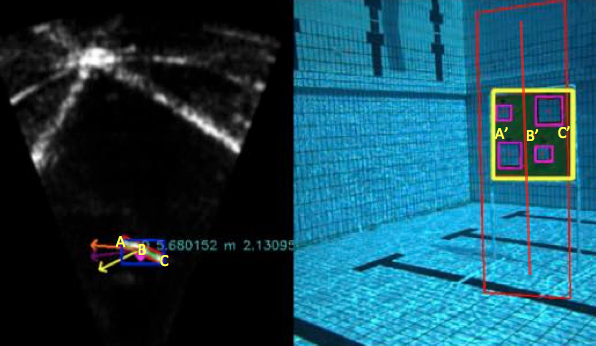
\includegraphics[scale=0.4]{project}
  \captionsetup{justification=centering}
  \caption{Matching objects in the sonar and camera by projecting ambiguity lines into the camera}
\end{figure}

This method has several drawbacks since matching both sonar and camera objects requires the ROI in the camera to be extracted accurately. While this method worked in pool conditions, it tended to fail in sea/lake conditions, due to particulate matter in water over large distances, or through temporal irradiance due to sunlight filtering through the water. Also, the vehicle's pitching motion tended to cause the intensity of the sonar object to drop as the object would go out of it's frustum, causing brief losses in detection. A framework was needed allow for consistent sensing of the object in 3D space.

\section{Particle Filter}

This is why the need of a statistical filter to track and localize these objects, constrained by the calibrated transformation between both the sonar and camera based on Eq. 20 is proposed and used. Since the objects being localized are stationary, it is also possible to involve the vehicle's odometry data in order to predict the position of these objects if loss in data occurred in the sonar or camera. 

\subsection{Dynamic Model}

The state matrix and dynamic model is given by Eq. 32 which represents the object position and velocity in 3D space in the sonar frame. $N$ number of particles representing possible solutions to where the object is are initially distributed over the workspace as per step 1. Then each particles position is updated based on a simple velocity displacement update matrix with some process noise $w_{k}$ added.
\begin{gather}
X_{n|n-1}^{(k)}=\left[\begin{array}{c}
X_{s}\\
Y_{s}\\
Z_{s}\\
\dot{X_{s}}\\
\dot{Y_{s}}\\
\dot{Z_{s}}
\end{array}\right]\quad X_{n|n-1}^{(k)}=\left[\begin{array}{cccccc}
1 & 0 & 0 & T & 0 & 0\\
0 & 1 & 0 & 0 & T & 0\\
0 & 0 & 1 & 0 & 0 & T\\
0 & 0 & 0 & 1 & 0 & 0\\
0 & 0 & 0 & 0 & 1 & 0\\
0 & 0 & 0 & 0 & 0 & 1
\end{array}\right]*X_{n-1|n-1}^{(k)}+w_{n-1}
\end{gather}

Since the object we are localizing is stationary w.r.t the world frame, we can incorporate the vehicle odometry into the object motion. This is so that if we are unable to measure (\XSonar, \YSonar, \ZSonar) in the measurement step, we can predict the object's next position based on the previous position and current velocity. To do this, we first transform $(X_{s},Y_{s,}Z_{s})_{k}$ at that time instant into the vehicle frame with the known ($L_{y}$, $L_{z}$), and convert it to polar coordinates, based on Eq. 33. We assume the sonar and vehicle frames have an identity rotational component here, and that ($L_{x}$) which cannot be estimated is minimal.
\begin{gather}
\left[\begin{array}{cccc}
1 & 0 & 0 & 0\\
0 & 1 & 0 & L_{y}\\
0 & 0 & 1 & L_{z}\\
0 & 0 & 0 & 1
\end{array}\right]*\left[\begin{array}{c}
X_{s}\\
Y_{s}\\
Z_{s}\\
1
\end{array}\right]_{k}=\left[\begin{array}{c}
X_{v}\\
Y_{v}\\
Z_{v}\\
1
\end{array}\right]_{k}=\left[\begin{array}{c}
R_{v}\cdot\cos\left(\phi_{v}\right)\cdot\sin\left(\theta_{v}\right)\\
R_{v}\cdot\sin\left(\phi_{v}\right)\\
R_{v}\cdot\cos\left(\phi_{v}\right)\cdot\cos\left(\theta_{v}\right)
\end{array}\right]
\end{gather}

We then differentiate the polar representation of the object in the vehicle frame in Eq. 33 to yield the Jacobian matrix in Eq. 34. 
\begin{gather}
\left[\begin{array}{c}
\dot{X_{v}}\\
\dot{Y_{v}}\\
\dot{Z_{v}}
\end{array}\right]=\frac{d}{dt}\left[\begin{array}{c}
R_{v}\cdot\cos\left(\phi_{v}\right)\cdot\sin\left(\theta_{v}\right)\\
R_{v}\cdot\sin\left(\phi_{v}\right)\\
R_{v}\cdot\cos\left(\phi_{v}\right)\cdot\cos\left(\theta_{v}\right)
\end{array}\right]= \nonumber\\
\left[\begin{array}{c}
\left(\dot{R_{v}}\cdot\cos\left(\phi_{v}\right)\cdot\sin\left(\theta_{v}\right)\right)-\left(R_{v}\cdot\dot{\phi_{v}}\cdot\sin\left(\phi_{v}\right)\cdot\sin\left(\theta_{v}\right)\right)+\left(R_{v}\cdot\dot{\theta_{v}}\cdot\cos\left(\phi_{v}\right)\cdot\cos\left(\theta_{v}\right)\right)\\
\left(\dot{R_{s}}\cdot\sin\left(\phi_{v}\right)\right)+\left(R_{v}\cdot\dot{\phi_{v}}\cdot\cos\left(\phi_{v}\right)\right)\\
\left(\dot{R_{v}}\cdot\cos\left(\phi_{v}\right)\cdot\cos\left(\theta_{v}\right)\right)-\left(R_{v}\cdot\dot{\phi_{v}}\cdot\sin\left(\phi_{v}\right)\cdot\cos\left(\theta_{v}\right)\right)-\left(R_{v}\cdot\dot{\theta_{v}}\cdot\cos\left(\phi_{v}\right)\cdot\sin\left(\theta_{v}\right)\right)
\end{array}\right]
\end{gather}

Next, some components in the Jacobian matrix are replaced with their equivalent readings of other sensors as seen in Eq. 35. The $\dot{R_{v}}$ components are equal to the negative vehicular translational velocity components, and the $\dot{\theta_{v}}$ and $\dot{\phi_{v}}$ are equal to the negative angular velocities of pitch and yaw. This yields Eq. 36, which shows the replaced values.
\begin{gather}
\left[\begin{array}{c}
\left(\dot{R_{v}}\cdot\cos\left(\phi_{v}\right)\cdot\sin\left(\theta_{v}\right)\right)\\
\left(\dot{R_{v}}\cdot\sin\left(\phi_{v}\right)\right)\\
\left(\dot{R_{v}}\cdot\cos\left(\phi_{v}\right)\cdot\cos\left(\theta_{v}\right)\right)
\end{array}\right]=\left[\begin{array}{c}
\dot{-X_{v}}\\
\dot{-Y_{v}}\\
\dot{-Z_{v}}
\end{array}\right]\quad\left[\begin{array}{c}
\dot{\theta_{v}}\\
\dot{\phi_{v}}
\end{array}\right]=\left[\begin{array}{c}
\dot{-\gamma_{v}}\\
\dot{-\beta_{v}}
\end{array}\right] \\
\left[\begin{array}{c}
\dot{X_{v}}\\
\dot{Y_{v}}\\
\dot{Z_{v}}
\end{array}\right]=\left[\begin{array}{c}
\left(\dot{-X_{v}}\right)-\left(R_{v}\cdot\dot{-\beta_{v}}\cdot\sin\left(\phi_{v}\right)\cdot\sin\left(\theta_{v}\right)\right)+\left(R_{v}\cdot\dot{-\gamma_{v}}\cdot\cos\left(\phi_{v}\right)\cdot\cos\left(\theta_{v}\right)\right)\\
\left(\dot{-Y_{v}}\right)+\left(R_{v}\cdot\dot{-\beta_{v}}\cdot\cos\left(\phi_{v}\right)\right)\\
\left(\dot{-Z_{v}}\right)-\left(R_{v}\cdot\dot{-\beta_{v}}\cdot\sin\left(\phi_{v}\right)\cdot\cos\left(\theta_{v}\right)\right)-\left(R_{v}\cdot\dot{-\gamma_{v}}\cdot\cos\left(\phi_{v}\right)\cdot\sin\left(\theta_{v}\right)\right)
\end{array}\right]
\end{gather}

We then perform the the update/prediction step based on the velocity model in Eq. 32, then transform the newly estimated $(X_{v},Y_{v},Z_{v})_{k+1}$ back into the sonar frame $(X_{s},Y_{s},Z_{s})_{k+1}$ as seen in Eq. 37.
\begin{gather}
\left[\begin{array}{cccc}
1 & 0 & 0 & 0\\
0 & 1 & 0 & -L_{y}\\
0 & 0 & 1 & -L_{z}\\
0 & 0 & 0 & 1
\end{array}\right]*\left[\begin{array}{c}
X_{v}\\
Y_{v}\\
Z_{v}\\
1
\end{array}\right]_{k+1}=\left[\begin{array}{c}
X_{s}\\
Y_{s}\\
Z_{s}\\
1
\end{array}\right]_{k+1}
\end{gather}

\subsection{Measurement Model}

Now that we have predicted the new position of the object (\XSonar, \YSonar, \ZSonar) using the dynamic model above, we wish to correct this with measurements from the sonar and camera. In order to do this, we project this data into their respective image pixels since their calibration data is known. Particles in the sonar frame are projected into the sonar image by converting (\XSonar, \YSonar, \ZSonar) into (\RSonar, \ThetaSonar, \PhiSonar) as seen in Eq. 38. \RSonar and \ThetaSonar may then be matched into the sonar image pixel coordinates provided by the Blueview API. (\XSonar, \YSonar, \ZSonar) are then transformed into the camera frame and projected into the camera based on the calibration data derived as seen in Eq. 39. From here, we can extract ($U_{s}, V_{s}$) and ($U_{c}, V_{c}$) pixel coordinates in both sensors from the particle state.
\begin{gather}
\left[\begin{array}{c}
\sqrt{X_{s}^{2}+Y_{s}^{2}+Z_{s}^{2}}\\
arctan(\frac{X_{s}}{Y_{s}})\\
arctan(\frac{Y_{s}}{\sqrt{X_{s}^{2}+Y_{s}^{2}+Z_{s}^{2}}})
\end{array}\right]=\left[\begin{array}{c}
R_{s}\\
\Theta_{s}\\
\Phi_{s}
\end{array}\right]=>\left[\begin{array}{c}
U_{s}\\
V_{s}
\end{array}\right] \\
\left[\begin{array}{cccc}
735.4809 & 0 & 388.9467 & 0\\
0 & 733.6047 & 292.0895 & 0\\
0 & 0 & 1 & 0
\end{array}\right]*\left[\begin{array}{cccc}
0.9993 & 0.0311 & 0.0219 & 0.1401\\
-0.0303 & 0.9989 & -0.0363 & 0.2671\\
-0.0230 & 0.0356 & 0.9991 & 0.1407\\
0 & 0 & 0 & 1
\end{array}\right]*
\left[\begin{array}{c}
X_{s}\\
Y_{s}\\
Z_{s}
\end{array}\right]=>\left[\begin{array}{c}
U_{c}\\
V_{c}
\end{array}\right]
\end{gather}

Computing the weight of the particles from the sonar image is done by taking ($U_{s}, V_{s}$) and testing that pixel against several features, such as brightness/intensity of that spot and major/minor axis of the shape of the object that pixel is in. This shape information such as the major/minor axis length is extracted by performing contour analysis, morphology and oriented bounding box fitting via Principle Component Analysis (PCA) \cite{Knauer2006}.

This is done by calculating the log likelihood of that particle/state where we assume the above features that are measured at a particular state follow a gaussian distribution given a user specified major/minor axis length. This is specified by Eq. 40/41. Here, $d$ represents the difference between a user specified measurement and actual measurement and $sigma$ represents the measurement standard deviation.
\begin{gather}
P(Y_{n}|X_{n|n-1}^{(k)})=\frac{1}{\sqrt{2\pi\sigma^{2}}}\cdot exp(-\frac{d^{2}}{2\sigma^{2}}) \\
log(P(Y_{n}|X_{n|n-1}^{(k)}))=-log(\sigma\sqrt{2\pi})-\frac{0.5}{\sigma^{2}}\cdot d^{2}
\end{gather}

The final sonar weight of a particle is given by Eq. 42 where Fig. 24 describes the features used.
\begin{gather}
q_{n}^{sonar}=-log(\sigma_{Intensity}\sqrt{2\pi})-\frac{0.5}{\sigma_{Intensity}^{2}}\cdot((U_{s},V_{s})_{Intensity}-255)^{2}+ \nonumber\\
-log(\sigma_{MajorAxis}\sqrt{2\pi})-\frac{0.5}{\sigma_{MajorAxis}^{2}}\cdot((U_{s},V_{s})_{MajorAxis}-User_{MajorAxis})^{2}+ \nonumber\\
-log(\sigma_{MinorAxis}\sqrt{2\pi})-\frac{0.5}{\sigma_{MinorAxis}^{2}}\cdot((U_{s},V_{s})_{MinorAxis}-User_{MinorAxis})^{2}
\end{gather}

\begin{figure}[h!]
  \centering
  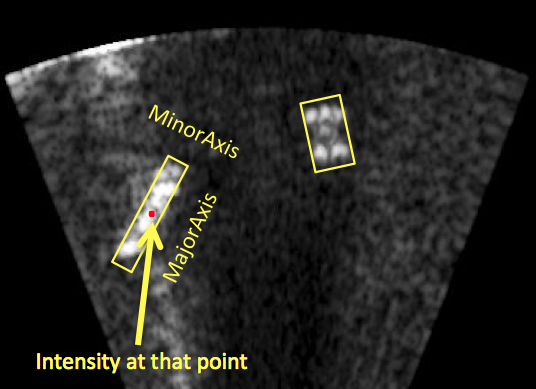
\includegraphics[scale=0.3]{majorminor}
  \captionsetup{justification=centering}
  \caption{Sonar Features used}
\end{figure}

Computing the weight of the particles from the camera image is done by taking ($U_{c}, V_{c}$) and testing that pixel against several features, such as hue and shape ratio. The final camera weight of a particle is given by Eq. 43.
\begin{gather}
q_{n}^{camera}=-log(\sigma_{Hue}\sqrt{2\pi})-\frac{0.5}{\sigma_{Hue}^{2}}\cdot((U_{c},V_{c})_{Hue}-User_{Hue})^{2}+ \nonumber\\
-log(\sigma_{Ratio}\sqrt{2\pi})-\frac{0.5}{\sigma_{Ratio}^{2}}\cdot((U_{c},V_{c})_{Ratio}-User_{Ratio})^{2}
\end{gather}

There is also the possibility of computing the Pixel Velocity using the Lucas-Kanade feature tracking method, and giving higher weights to the projected particles that match this velocity, but using the above features were found to be sufficient. We finally add these weights up, perhaps giving more weightage to either sensor in the fusion process if the user requires it, and normalize it as per step 4. Resampling with replacement is then applied as per step 5 and the process is repeated. Finally, in order to extract results from the state matrix, we use GMM (Gaussian Mixture Model) clustering to extract the mean and covariance of the particle clusters.
\begin{gather}
P(Y_{n}|X_{n|n-1}^{(k)})=q_{n}^{sonar}+q_{n}^{camera} \\
q_{n}=\frac{P(Y_{n}|X_{n|n-1}^{(k)})}{\sum_{k}P(Y_{n}|X_{n|n-1}^{(k)})}\quad k\epsilon\mathbb{N}
\end{gather}

\subsection{Particle Filter Results}

Fig. 27 to Fig. 29 shows the particle filter algorithm in action tested in pool conditions. One can observe that initially, there is ambiguity in \PhiSonar as the object wasn't visible in the camera. As the vehicle moves closer, the ambiguity is corrected. Finally, as the object moves out of the sonar image, we can see the ambiguity in \RSonar. Also, in instances wgere there is loss of information from either sensor, we are still able to predict the next position of the object using the vehicle odometry data.

Fig. 30 to Fig. 32 show the particle filter algorithm in action tested in murky water conditions with poor visibility in the camera imagery, and a low SNR in the sonar imagery due to the object being almost out of the sonar frustum as seen in Fig. 31. Despite this, the particles still converge on the correct solution over time. It is also impervious to noise from surrounding wall as seen in Fig. 32. 

We can see the mapping vs particle filter localization results on Fig. 34 for both cases. The graph on the left shows the (\XSonar,\YSonar,\ZSonar) axis measurements gotten from both the mapping algorithm described in section 3.4 and the particle filter algorithm over time. The figure on the right shows the same data but represented in 3D space. The mapping algorithm loses a lot of data points as it requires testing the ROI extracted from the camera against the projected ROI of the sonar object. This method still worked well in the first case in pool conditions, but failed miserably in murky water conditions, with intermittent data loss and noisy data points. Using the particle filter method however, we can observe much better results that fill in a lot of the gaps of the first method and are much smoother.

\section{Conclusion}
This paper proposed a novel object localization algorithm in the 3D space in front of the AUV using particle filters, where the calibration parameters between the sonar and camera are used to enforce a model constraint. The algorithm was validated through implementation as a real time system on the BumbleBee Autonomous Underwater Vehicle (BBAUV).
 
The resulting algorithm was found to meet the specifications and objectives stated in the beginning of the project. The localization of objects in 3D space using the sonar and camera outperforms methods using only 1 sensor alone. 
 
Future work can be done to possibly better estimate the complete transformation between all frames in the vehicle, include $L_{x}$, by incorporating the vehicular odometry data in the calibration model. Extracting precise ground truth is also a challenge, as GPS is unable to work underwater and odometry data from the DVL may not be precise enough. Rather than relying on data from the camera and depth sensor for ground truth, better methods such as long baseline (LBL) acoustic positioning systems may be considered. Lastly, working from a world frame instead of vehicle/object frame may be considered in the future, so that it may be easily extended to SLAM frameworks. 


% Figures
\clearpage
\newpage
\FloatBarrier
\begingroup\setlength{\belowcaptionskip}{-2pt}
\section{Figures}

\begin{figure*}[!htbp]
  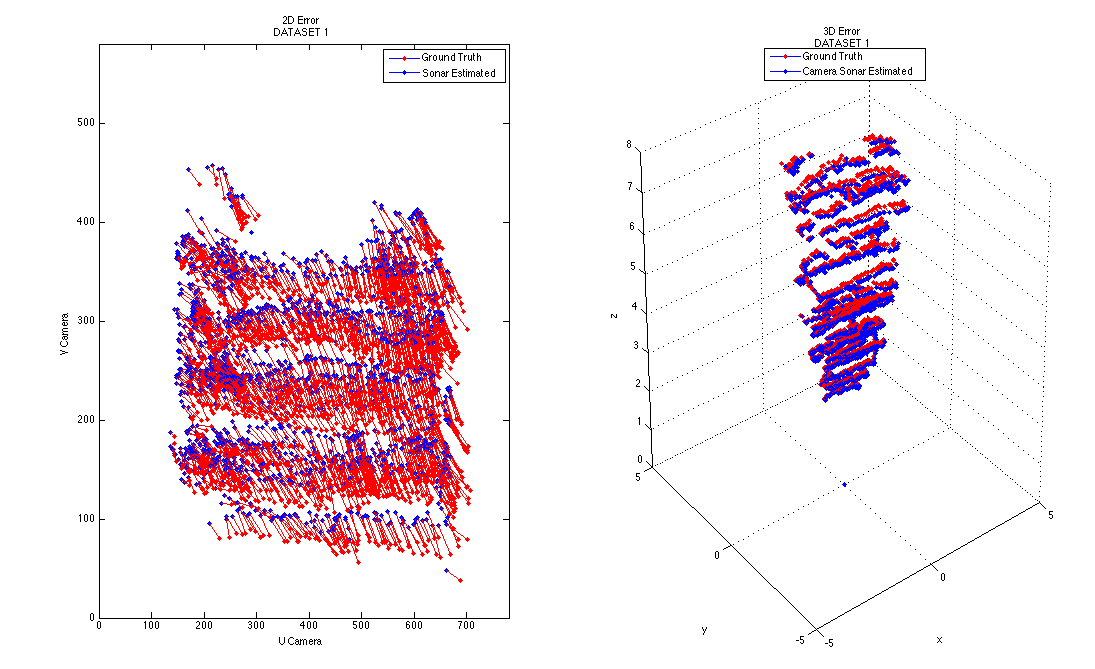
\includegraphics[width=\textwidth,height=8cm]{1}
  \caption{Large errors in pixel space (left) and 3D space (right) before calibration}
\end{figure*}

\begin{figure*}[!htbp]
  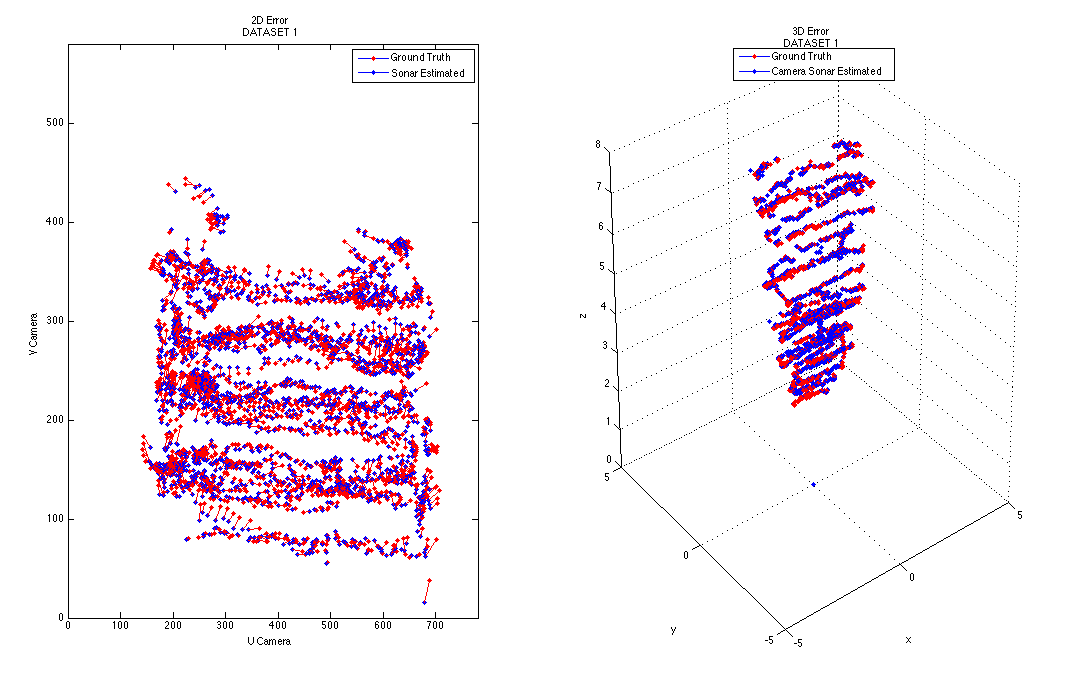
\includegraphics[width=\textwidth,height=8cm]{4}
  \caption{Reduced errors in pixel space (left) and 3D space (right) after calibration}
\end{figure*}

\begin{figure*}[!htbp]
\centering
\begin{subfigure}{\columnwidth}
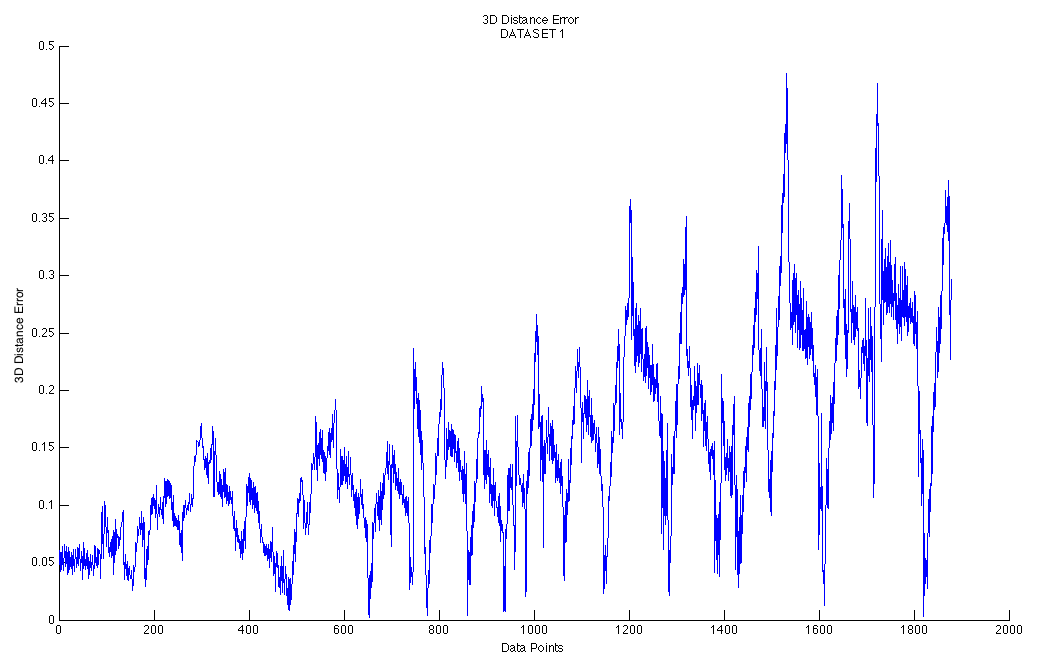
\includegraphics[width=\columnwidth]{3}%
\caption{Mean 3D Euclidean error of approx 15cm on training set before calibration}%
\label{subfiga}%
\end{subfigure}\hfill%
\begin{subfigure}{\columnwidth}
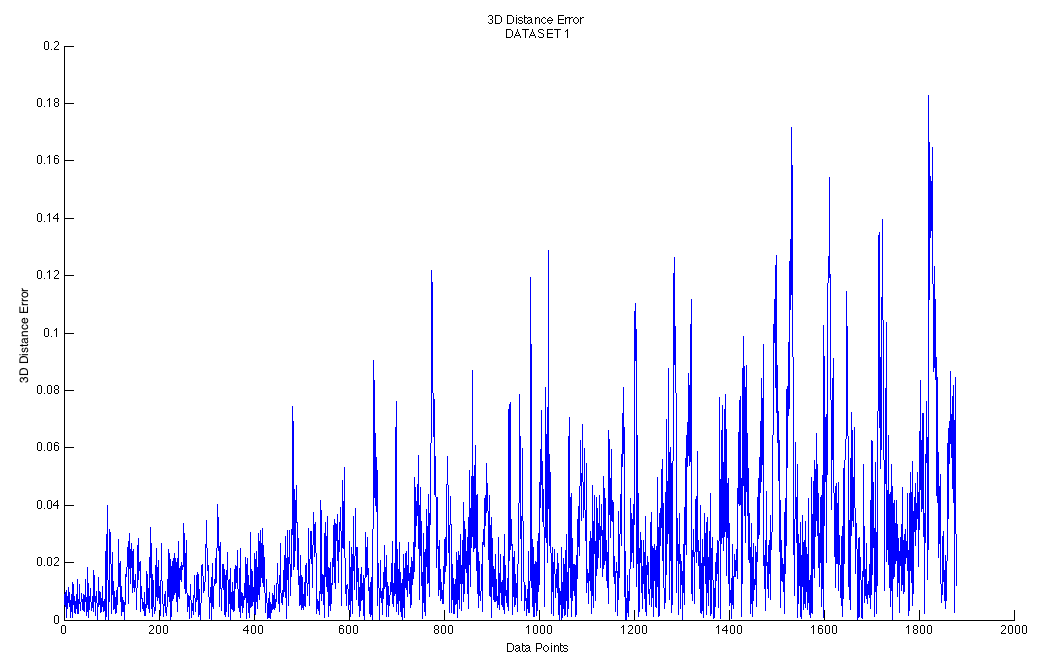
\includegraphics[width=\columnwidth]{6}%
\caption{Mean 3D Euclidean error of approx 2cm on training set after calibration}%
\label{subfiga}%
\end{subfigure}\hfill%
\caption{3D Euclidean error between resolved 3D coordinates from sonar and camera data vs ground truth in metres}
\label{figabc}
\end{figure*}

\begin{figure*}[!htbp]
  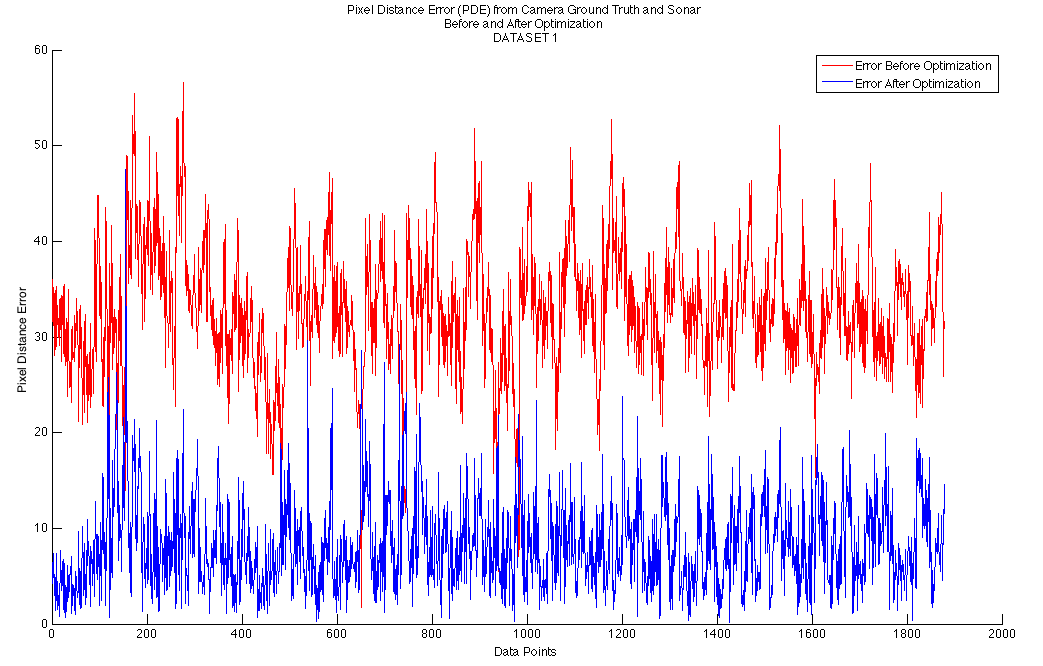
\includegraphics[width=\textwidth,height=10cm]{5}
  \caption{2D Pixel Euclidean error between projected pixels and ground truth before and after calibration}
\end{figure*}

\begin{figure*}[!htbp]
\centering
\begin{subfigure}{\columnwidth}
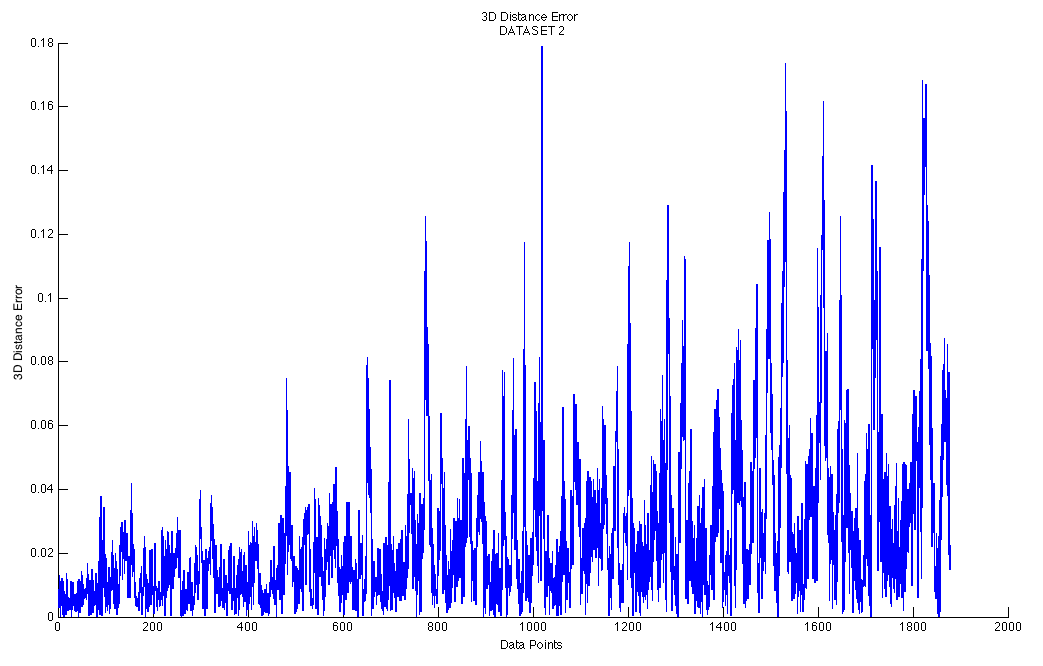
\includegraphics[width=\columnwidth]{T2}%
\caption{3D Euclidean error Test Set 2}%
\label{subfiga}%
\end{subfigure}\hfill%
\begin{subfigure}{\columnwidth}
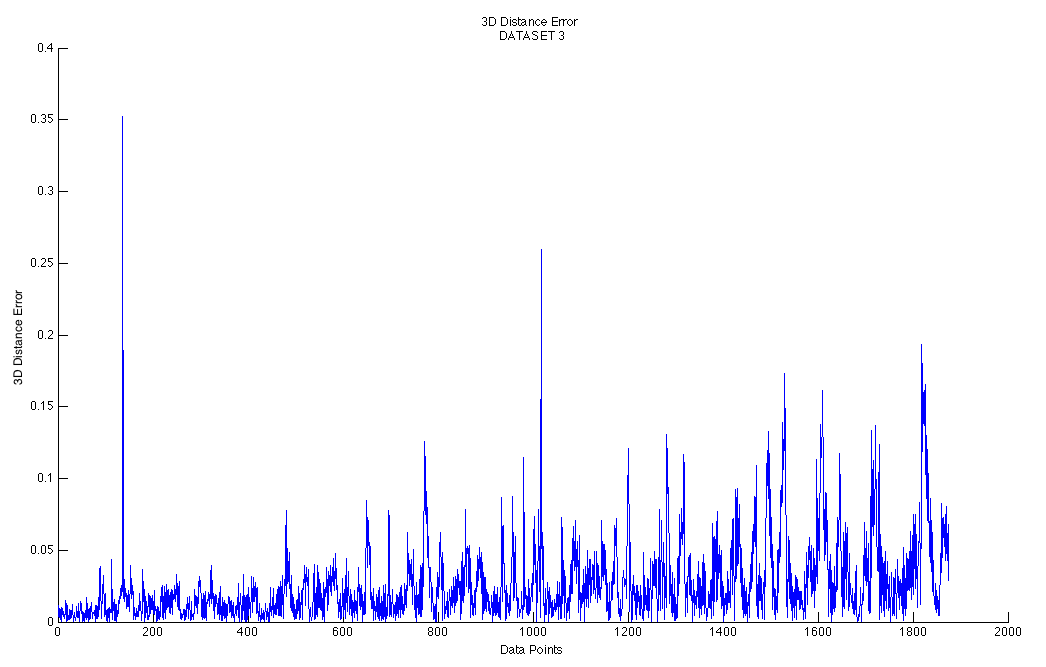
\includegraphics[width=\columnwidth]{T3}%
\caption{3D Euclidean error Test Set 3}%
\label{subfiga}%
\end{subfigure}\hfill%
\end{figure*}
\begin{figure*}%
\centering
\begin{subfigure}{\columnwidth}
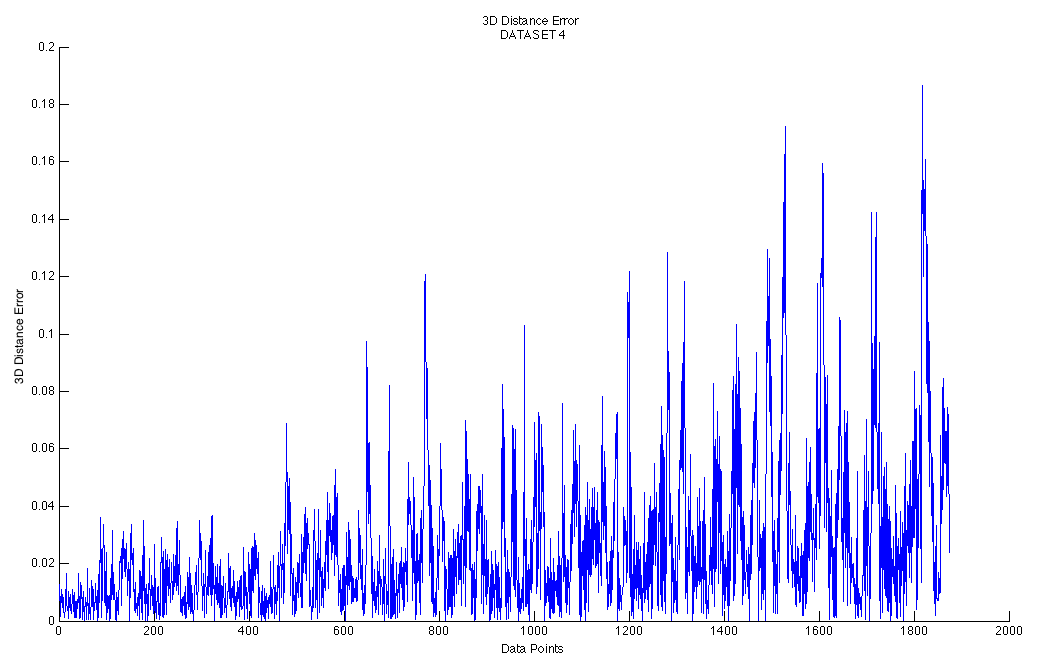
\includegraphics[width=\columnwidth]{T4}%
\caption{3D Euclidean errorTest Set 4}%
\label{subfiga}%
\end{subfigure}\hfill%
\begin{subfigure}{\columnwidth}
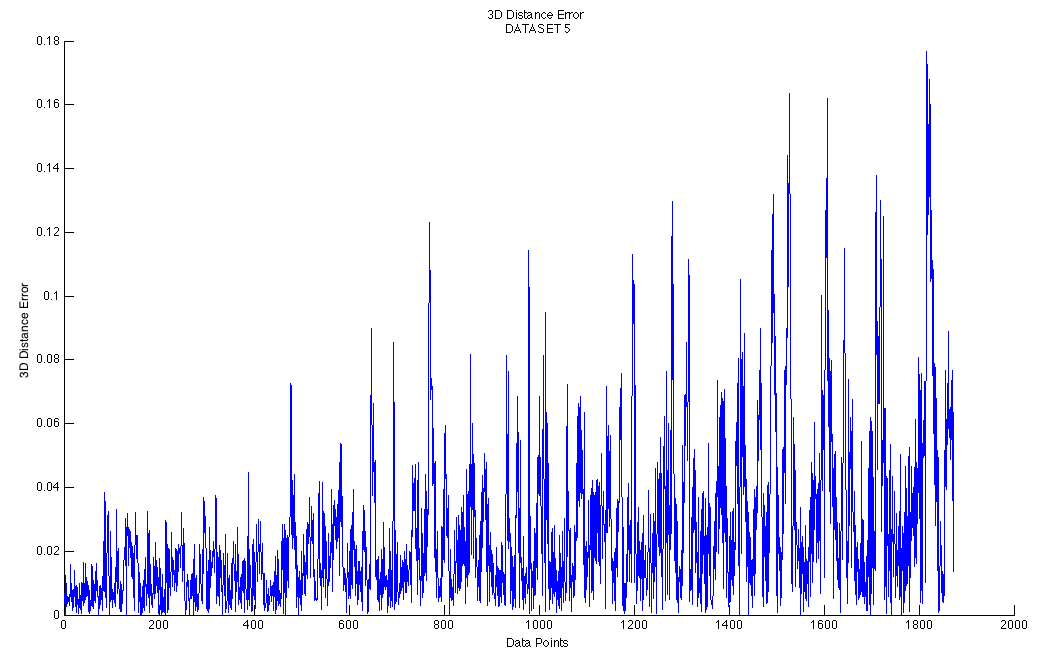
\includegraphics[width=\columnwidth]{T5}%
\caption{3D Euclidean error Test Set 5}%
\label{subfiga}%
\end{subfigure}\hfill%
\caption{Testing calibrated parameters derived from training set against 4 test sets}
\label{figabc}
\end{figure*}

\begin{figure*}
  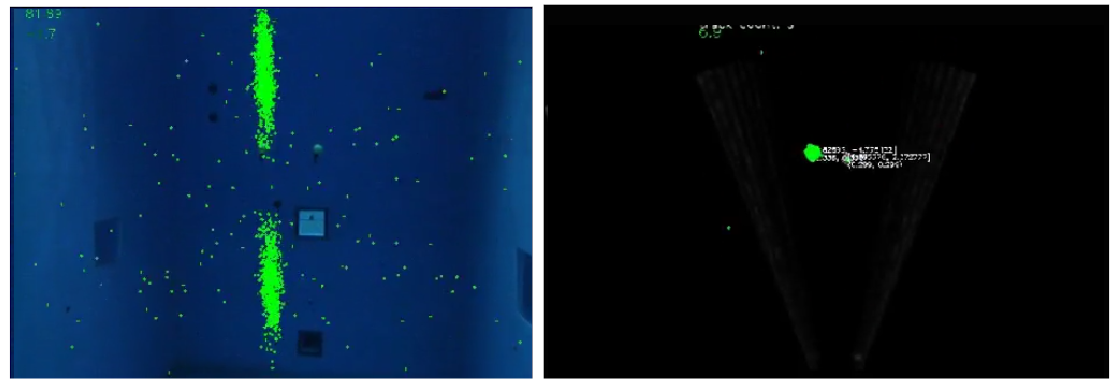
\includegraphics[width=\textwidth,height=7cm]{pfraw3}
  \caption{Object not visible in camera, hence bigger uncertainty in elevation as seen in the camera image}
  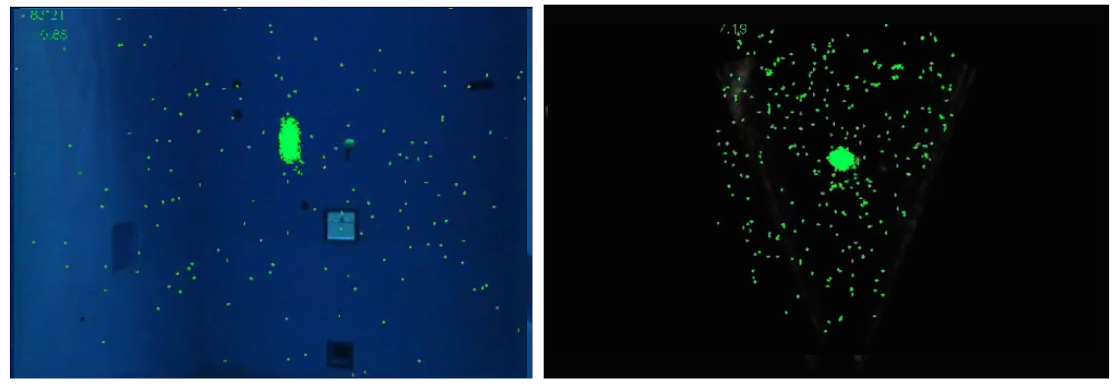
\includegraphics[width=\textwidth,height=7cm]{pfraw4}
  \captionsetup{font=small,skip=-10pt,justification=centering}
  \caption{Elevation ambiguity corrected via camera. Also loss of sonar information at that instant, but position still maintained through camera and odometry fusion but with increased covariance}
  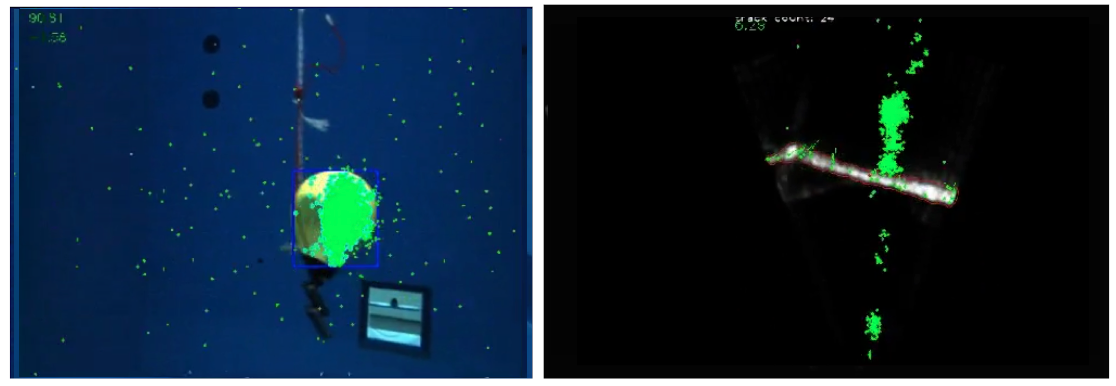
\includegraphics[width=\textwidth,height=7cm]{pfraw5}
  \captionsetup{font=small,skip=-10pt,justification=centering}
  \caption{Object not visible in sonar, hence ambiguity in range}
\end{figure*}

\begin{figure*}
  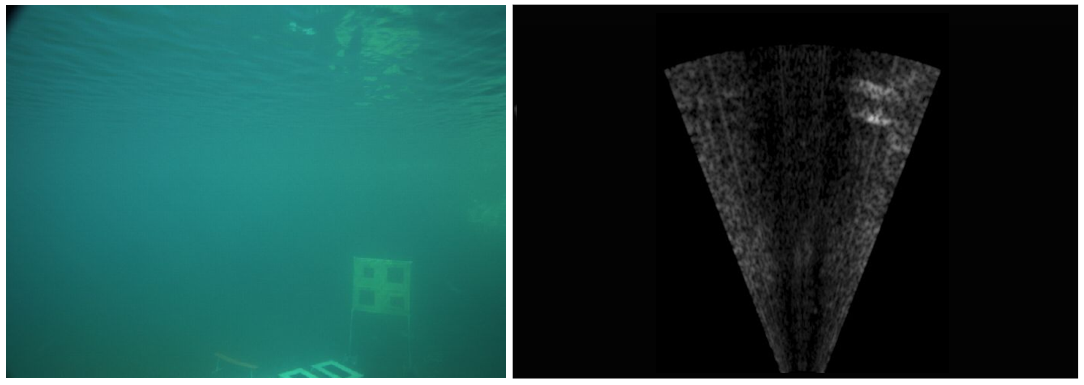
\includegraphics[width=\textwidth,height=7cm]{pfsem1}
  \caption{Objective is to localize the task board located nearly 15m away in murky water and is barely visible in either sensor}
  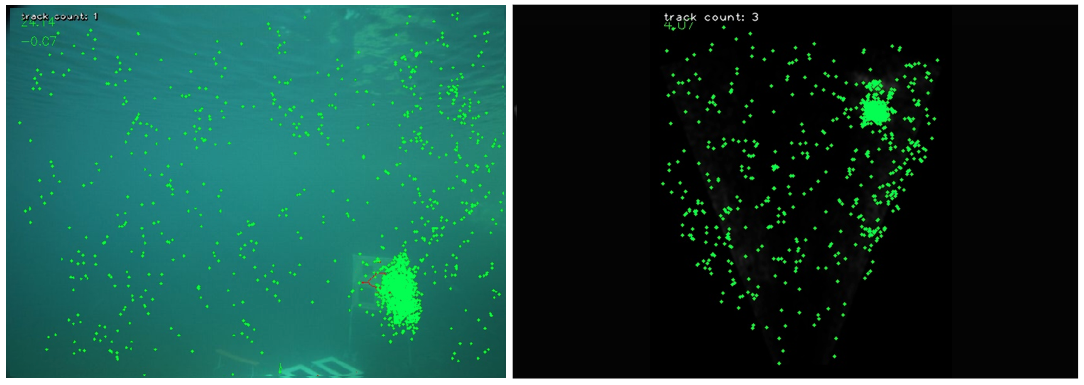
\includegraphics[width=\textwidth,height=7cm]{pfsem2}
  \caption{Particle Filter still localizes the object in 3D space}
  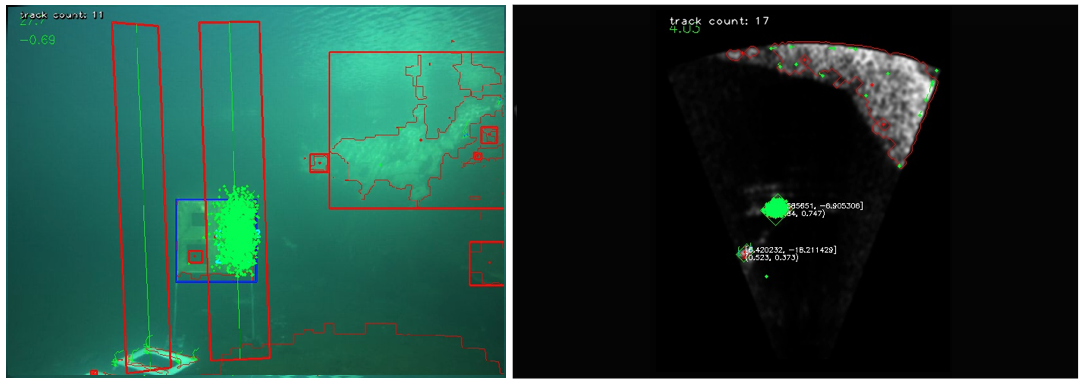
\includegraphics[width=\textwidth,height=7cm]{pfsem3}
  \captionsetup{font=small,skip=-10pt,justification=centering}
  \caption{Particle Filter localizes the object despite noisy data in both sensors when close to a wall}
\end{figure*}

\begin{figure*}%
\centering
\begin{subfigure}{\columnwidth}
\centering
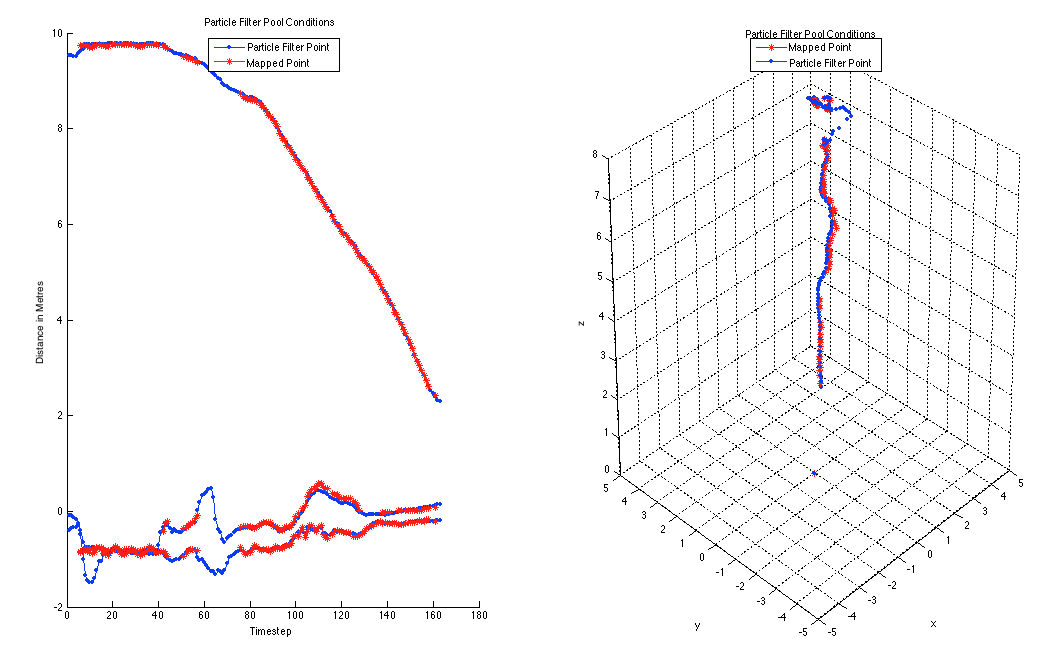
\includegraphics[width=0.9\columnwidth]{gg}%
\caption{Pool conditions}%
\end{subfigure}\hfill%
\begin{subfigure}{\columnwidth}
\centering
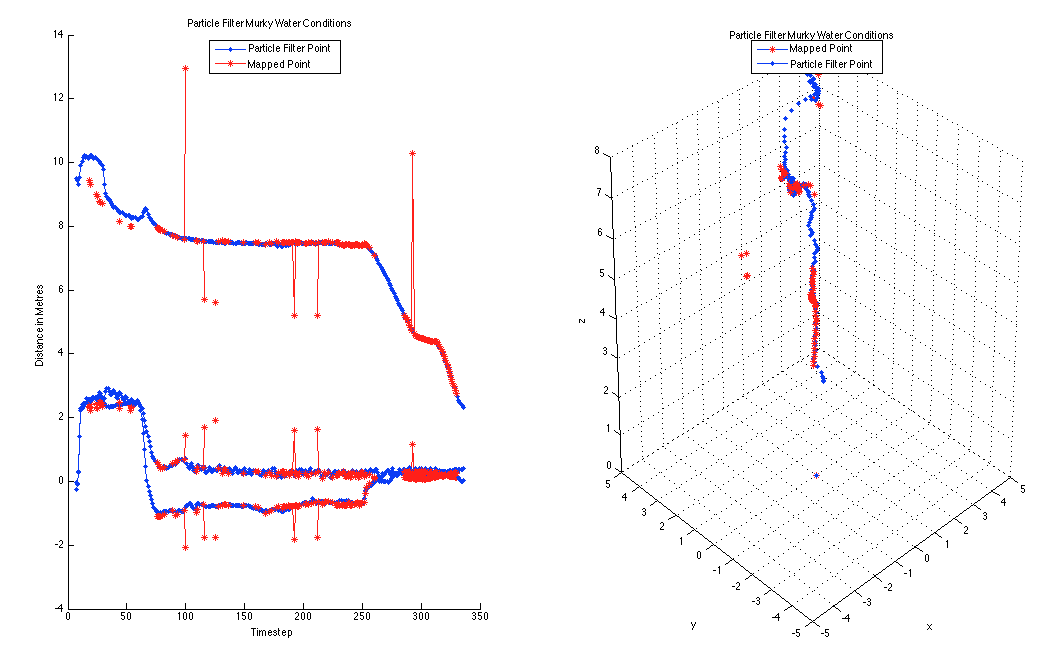
\includegraphics[width=0.9\columnwidth]{gg2}%
\caption{Murky water conditions}%
\label{subfiga}%
\end{subfigure}\hfill%
\end{figure*}
\begin{figure*}%
\centering
\caption{Comparison of object coordinates derived through the mapping method vs particle filter}
\label{figabc}
\end{figure*}
\endgroup

% References
\clearpage
\bibliographystyle{plain}
\bibliography{test}

\end{document}